\documentclass[12pt,a4paper]{article}

% ---------- Codificación e idioma ----------
\usepackage[utf8]{inputenc}
\usepackage[T1]{fontenc}
\usepackage[spanish,es-noshorthands]{babel}
\usepackage{lmodern}

% ---------- Paquetes útiles ----------
\usepackage[margin=2.5cm]{geometry}
\usepackage{graphicx}
\usepackage{xcolor}
\usepackage{booktabs}
\usepackage{array}
\usepackage{enumitem}
\usepackage{parskip}
\usepackage{verbatim}
\usepackage{longtable}   % tablas que ocupan más de una página
\usepackage{listings}    % código y salidas del notebook
\usepackage[hidelinks]{hyperref}
\usepackage{xurl}   % permite cortar las URLs largas para que no se salgan del margen

% ---------- Referencias con sangria francesa (APA) ----------
\newenvironment{referencias}
  {\begin{list}{}{%
     \setlength{\leftmargin}{1.6em}\setlength{\itemindent}{-1.6em}%
     \setlength{\labelwidth}{0pt}\setlength{\labelsep}{0pt}%
     \setlength{\itemsep}{0.7em}\setlength{\parsep}{0pt}}}
  {\end{list}}

% ---------- Colores ----------
\definecolor{azulUVG}{RGB}{30,90,150}
\definecolor{verde}{RGB}{46,139,87}
\definecolor{grisclaro}{RGB}{240,243,246}
\definecolor{gristexto}{RGB}{90,100,110}

% ---------- Caracteres que no trae la fuente ----------
\DeclareUnicodeCharacter{2605}{\ensuremath{\star}}
\DeclareUnicodeCharacter{2192}{\ensuremath{\rightarrow}}

% ---------- Estilo del código y de las salidas del notebook ----------
\lstdefinestyle{base}{
  basicstyle=\ttfamily\footnotesize,
  columns=fullflexible, keepspaces=true, showstringspaces=false, upquote=true,
  breaklines=true, postbreak=\mbox{\textcolor{gristexto}{$\hookrightarrow$}\space},
  aboveskip=0.6em, belowskip=0.9em, xleftmargin=6pt, xrightmargin=6pt,
  literate=
    {á}{{\'a}}1 {é}{{\'e}}1 {í}{{\'i}}1 {ó}{{\'o}}1 {ú}{{\'u}}1
    {Á}{{\'A}}1 {É}{{\'E}}1 {Í}{{\'I}}1 {Ó}{{\'O}}1 {Ú}{{\'U}}1
    {ñ}{{\~n}}1 {Ñ}{{\~N}}1 {ü}{{\"u}}1 {ç}{{\c{c}}}1 {ï}{{\"i}}1
    {¿}{{?`}}1 {¡}{{!`}}1 {·}{{\textperiodcentered}}1
    {—}{{\textemdash}}1 {–}{{\textendash}}1 {…}{{\ldots}}1
    {→}{{$\rightarrow$}}1 {★}{{$\star$}}1
}
\lstdefinestyle{codigo}{
  style=base, language=Python, deletekeywords={as},
  backgroundcolor=\color{grisclaro}, frame=single, rulecolor=\color{grisclaro}, framesep=5pt,
  keywordstyle=\color{azulUVG}\bfseries, stringstyle=\color{verde},
  commentstyle=\color{gristexto}\itshape,
}
\lstdefinestyle{salida}{
  style=base, basicstyle=\ttfamily\scriptsize,
  frame=leftline, rulecolor=\color{azulUVG}, framerule=1.5pt, framesep=6pt,
}

% Secciones sin numerar para un estilo menos formal
\setcounter{secnumdepth}{0}
\pagestyle{plain}

\begin{document}

% =====================================================================
%  CARÁTULA
% =====================================================================
\begin{titlepage}
\begin{center}

\textbf{UNIVERSIDAD DEL VALLE DE GUATEMALA}\\
Facultad de Ingeniería\\[2cm]

\IfFileExists{logo uvg.png}{%
  
\includegraphics[width=0.35\textwidth]{logo uvg.png}\\[2.5cm]
}{%
  \vspace*{2.5cm}
}

{\LARGE\textbf{Laboratorio 4: Extracción lingüística con Hugging Face}}\\[0.6cm]
{\large Sentimiento y entidades nombradas en reseñas de Barça Cafe}\\[1.5cm]

Diego Linares\\[0.2cm]


Procesamiento de Lenguaje Natural\\[2cm]

Septiembre de 2026

\end{center}
\end{titlepage}


% ---------------------------------------------------
\section{Introducción}

¿Qué tan bien funcionan los modelos preentrenados de Hugging Face cuando se les da reseñas reales
en español, sin ajustar nada?

Para responderlo se construyó un pipeline con \texttt{transformers} (Wolf et al., 2020) sobre
reseñas de \textbf{Barça Cafe}, el restaurante oficial del FC Barcelona junto al Spotify Camp Nou.
El pipeline clasifica el sentimiento de cada reseña (Parte A), extrae entidades nombradas
(Parte B), junta ambas salidas en una estructura por reseña (Parte C), calcula estadísticas y
exporta \texttt{laboratorio\_4\_resultados.csv} (Parte D), y analiza los casos en los que el modelo
se equivoca (Parte E).

El restaurante no se eligió al azar. En Google Maps tiene 3.2 estrellas con opiniones muy
polarizadas: a mucha gente le encanta la decoración y a mucha otra le parece caro y mediocre. Eso
garantiza reseñas positivas, negativas y mixtas, que es justo lo que pide la guía.

Este documento es el notebook \texttt{laboratorio\_4\_barca\_cafe.ipynb} en formato de reporte:
se incluyen las celdas de código, sus salidas y el análisis. Las tablas muy anchas del notebook se
presentan aquí como tablas de \LaTeX{} con las mismas cifras. El código completo está en
\url{https://github.com/DiegoLinares11/LAB-4-Extraccion-Linguistica-Con-Hugging-Face}.


% ---------------------------------------------------
\section{1. Dataset}

Las reseñas se basan en la ficha de Barça Cafe en Google Maps (Carrer d'Arístides Maillol 12,
Les Corts, Barcelona), consultada el 14 de septiembre de 2026 (Google, s.f.). Tiene
\textbf{3.2 estrellas con 424 opiniones} y esta distribución:

\begin{center}
\renewcommand{\arraystretch}{1.4}
\begin{tabular}{|l|r|r|r|r|r|}
\hline
\textbf{Estrellas} & \textbf{5} & \textbf{4} & \textbf{3} & \textbf{2} & \textbf{1} \\
\hline
Opiniones & 176 & 33 & 34 & 44 & 137 \\
\hline
\end{tabular}
\end{center}

\subsection{Por qué no se copiaron las reseñas literales}

La guía pide no incluir datos personales reales, y una reseña de Google Maps no es solo texto:
trae el nombre del autor, su foto, su perfil de \emph{Local Guide} y la fecha. Además el texto
pertenece a quien lo escribió, y los Términos de Servicio de Google Maps no permiten extraer ese
contenido para reutilizarlo. Por eso el dataset se armó así:

\begin{itemize}[leftmargin=1.2em]
\item \textbf{6 reseñas son paráfrasis} de las opiniones que Google Maps muestra públicamente:
los tres fragmentos destacados del resumen y las tres reseñas visibles sin iniciar sesión. Se
reescribieron con otras palabras y sin autor, conservando la opinión: café frío, café caro y
baños sucios, vaso de plástico cobrado sin avisar, hamburguesa ``1/10'', camareras amables,
comida exquisita.
\item \textbf{30 reseñas son simuladas} a partir de los temas reales que Google detecta en las 424
opiniones: \emph{hamburguesa} (54 menciones), \emph{barça} (41), \emph{mesa} (18),
\emph{cerveza} (16), \emph{estadio} (10), \emph{baños} (9), \emph{vaso de plástico} (7).
\item \textbf{Todos los nombres de clientes y empleados son ficticios} (Nuria, Sergi, Santiago,
Mateo). Se mantienen organizaciones y lugares públicos (FC Barcelona, Real Madrid, Les Corts,
Guatemala) y dos referencias públicas del restaurante: el jugador Lamine Yamal y los hermanos
Iglesias, a quienes el club anunció como responsables de la carta (FC Barcelona, 2021). No son
datos privados y hacen falta para probar el NER con personas.
\end{itemize}

\subsection{Etiqueta humana y cobertura}

Antes de correr cualquier modelo, a cada reseña se le asignó una \texttt{etiqueta\_humana} y una
lista de \texttt{casos}. Esa etiqueta es la referencia contra la que se comparan los modelos.

\begin{lstlisting}[style=codigo]
df_resenas = pd.read_csv(DATOS)
assert len(df_resenas) >= 30, "La guía pide un mínimo de 30 reseñas"

print(f"{len(df_resenas)} reseñas  |  columnas: {list(df_resenas.columns)}\n")
df_resenas[["review_id", "text", "etiqueta_humana", "estrellas", "casos"]]
\end{lstlisting}

\begin{lstlisting}[style=salida]
36 reseñas  |  columnas: ['review_id', 'text', 'etiqueta_humana', 'estrellas', 'casos', 'tema', 'origen']
\end{lstlisting}

\begin{lstlisting}[style=codigo]
cobertura = (df_resenas.assign(caso=df_resenas["casos"].str.split(";"))
             .explode("caso")["caso"].value_counts().rename("reseñas"))

print("Etiqueta humana:")
print(df_resenas["etiqueta_humana"].value_counts().to_string(), "\n")
print("Origen:")
print(df_resenas["origen"].value_counts().to_string(), "\n")
print("Tipos de caso cubiertos:")
print(cobertura.to_string())
\end{lstlisting}

\begin{center}\small\renewcommand{\arraystretch}{1.25}
\begin{tabular}[t]{|l|r|}\hline\textbf{Etiqueta humana} & \textbf{Reseñas} \\ \hline
POSITIVO & 15 \\ \hline
NEGATIVO & 14 \\ \hline
MIXTO & 5 \\ \hline
NEUTRO & 2 \\ \hline
\end{tabular}\qquad
\begin{tabular}[t]{|l|r|}\hline\textbf{Tipo de caso} & \textbf{Reseñas} \\ \hline
\texttt{entidades} & 14 \\ \hline
\texttt{positivo} & 9 \\ \hline
\texttt{negativo} & 7 \\ \hline
\texttt{negacion} & 6 \\ \hline
\texttt{mixto} & 5 \\ \hline
\texttt{texto\_corto} & 4 \\ \hline
\texttt{sarcasmo} & 3 \\ \hline
\texttt{error\_ortografico} & 2 \\ \hline
\texttt{neutro} & 2 \\ \hline
\texttt{mixto\_leve} & 1 \\ \hline
\texttt{entidad\_desconocida} & 1 \\ \hline
\texttt{jerga} & 1 \\ \hline
\texttt{mezcla\_idiomas} & 1 \\ \hline
\end{tabular}\end{center}


El dataset completo (36 reseñas) queda así; ``Hum.'' es la etiqueta humana y ``Est.'' la
estrella simulada:

{\footnotesize\setlength{\tabcolsep}{4pt}\renewcommand{\arraystretch}{1.25}
\begin{longtable}{|>{\raggedright\arraybackslash}p{0.55cm}|>{\raggedright\arraybackslash}p{9.0cm}|>{\raggedright\arraybackslash}p{1.25cm}|>{\raggedright\arraybackslash}p{0.6cm}|>{\raggedright\arraybackslash}p{3.0cm}|}
\hline
\textbf{ID} & \textbf{Reseña} & \textbf{Hum.} & \textbf{Est.} & \textbf{Casos} \\ \hline
\endfirsthead
\hline
\textbf{ID} & \textbf{Reseña} & \textbf{Hum.} & \textbf{Est.} & \textbf{Casos} \\ \hline
\endhead
1 & Fuimos después del tour del Museo del FC Barcelona y nos encantó. La decoración azulgrana, las pantallas gigantes y unos camareros muy agradables. Muy recomendable. & POS & 5 & positivo, entidades \\ \hline
2 & La camarera Nuria nos atendió de maravilla, súper simpática y rápida. La comida muy rica y el sitio precioso. & POS & 5 & positivo, entidades \\ \hline
3 & Pedí dos cafés y un croissant de chocolate y me lo sirvieron todo frío. Para estar dentro del estadio esperaba bastante más. & NEG & 1 & negativo \\ \hline
4 & Tres euros y medio por un café mediocre. Encima los baños estaban sucios a mediodía de un martes cualquiera. El FC Barcelona debería cuidar más sus instalaciones. & NEG & 1 & negativo, entidades \\ \hline
5 & El chico de la caja fue muy amable, eso sí. Lo que me molestó es que te cobran el vaso de plástico sin avisarte ni darte otra opción. & MIX & 2 & mixto \\ \hline
6 & Voy probando hamburguesas por todo Barcelona y esta es de las peores: pan seco y carne sin sabor. Un 1 sobre 10. & NEG & 1 & negativo, entidades \\ \hline
7 & Un sitio precioso para visitar, la comida riquísima y el personal muy atento. & POS & 5 & positivo \\ \hline
8 & Vimos el clásico del Barça contra el Real Madrid en las pantallas gigantes. Ambiente espectacular y la Estrella Damm bien fría. & POS & 5 & positivo, entidades \\ \hline
9 & Genial, 40 minutos esperando una hamburguesa que llegó fría. Una experiencia inolvidable, de verdad. & NEG & 1 & sarcasmo \\ \hline
10 & No volvería. No es que la comida sea horrible, pero no vale lo que cuesta. & NEG & 2 & negacion \\ \hline
11 & No está nada mal para ser un sitio turístico. Las bravas no tienen nada que envidiar a las de cualquier bar de Les Corts. & POS & 4 & negacion, entidades \\ \hline
12 & Top!! & POS & 5 & texto corto \\ \hline
13 & Carísimo. & NEG & 1 & texto corto \\ \hline
14 & La decoración con camisetas firmadas y lámparas en forma de balón es preciosa, pero la comida es muy normalita y cara. & MIX & 3 & mixto \\ \hline
15 & no bale la pena, la amburguesa estava cruda i el refresco sin gas. nunca mas & NEG & 1 & error ortografico, negacion \\ \hline
16 & q buen sitio!! los nachos buenisimos y el camarero super atento, bolveremos seguro & POS & 5 & error ortografico \\ \hline
17 & Está junto al Palau Blaugrana, en la calle Arístides Maillol. Abren a las 10 de la mañana. & NEU & 3 & neutro, entidades \\ \hline
18 & Vinimos desde Guatemala solo para conocer el Spotify Camp Nou y comer aquí fue la guinda. Mi hijo Santiago salió feliz con su camiseta de Lamine Yamal. & POS & 5 & positivo, entidades \\ \hline
19 & La carta la diseñaron los hermanos Iglesias y se nota en algunos platos, pero el servicio no está a la altura: tardaron muchísimo. & MIX & 3 & mixto, entidades \\ \hline
20 & Nos tuvieron esperando de pie aunque había mesas libres. Cuando por fin nos sentamos, la mesa estaba pegajosa. & NEG & 1 & negativo \\ \hline
21 & Buena opción para comer algo rápido antes del partido. Precios de estadio, pero la calidad es correcta y el personal eficiente. & POS & 4 & positivo, mixto leve \\ \hline
22 & Qué suerte tenemos los culés: pagar siete euros por una cerveza en vaso de plástico. Así seguro que terminan la reforma del estadio. & NEG & 2 & sarcasmo \\ \hline
23 & Los camareros son un amor, pero la cocina es un desastre: el pollo seco y las patatas congeladas. & MIX & 2 & mixto \\ \hline
24 & Celebramos el cumpleaños de mi sobrino Mateo aquí y el equipo del Barça Cafe se portó genial, hasta le pusieron una vela en el postre. & POS & 5 & positivo, entidades \\ \hline
25 & Personal desbordado, música altísima y nadie limpió nuestra mesa en toda la tarde. Una pena para la imagen del club. & NEG & 1 & negativo \\ \hline
26 & Meh. & NEG & 2 & texto corto \\ \hline
27 & No puedo decir que no me haya gustado: el bocadillo de jamón estaba bueno y no tardaron nada. & POS & 4 & negacion \\ \hline
28 & Esperaba algo digno del Museu del Barça y me encontré un bar de aeropuerto con precios de Plaça de Catalunya. & NEG & 1 & negativo, entidades \\ \hline
29 & La Blaugrana Burger con salsa Culé está brutal, pídanla sin dudar. & POS & 5 & entidad desconocida, jerga \\ \hline
30 & Amazing ambiente, la paella muy good y el staff very friendly. ¡Volveremos desde México! & POS & 5 & mezcla idiomas, entidades \\ \hline
31 & Pedí una ensalada y me trajeron una hamburguesa. Cuando lo reclamé, el encargado Sergi ni se disculpó. & NEG & 1 & negativo, entidades \\ \hline
32 & Para ver un partido con amigos está bien, para comer no lo recomiendo. & MIX & 3 & mixto, negacion \\ \hline
33 & El brunch del domingo fue una sorpresa: huevos benedictinos riquísimos, zumo natural y vistas al estadio. & POS & 5 & positivo \\ \hline
34 & Cinco estrellas... para el aire acondicionado, que es lo único que funcionaba. & NEG & 1 & sarcasmo \\ \hline
35 & Normal. Ni bueno ni malo. & NEU & 3 & neutro, negacion, texto corto \\ \hline
36 & Coincidimos con aficionados de Japón y Brasil y acabamos todos cantando el himno del Barça. Ambiente único en Barcelona. & POS & 5 & positivo, entidades \\ \hline
\end{longtable}}


% ---------------------------------------------------
\section{2. Configuración}

La primera celda instala solo las dependencias que falten, para que el notebook corra igual en
Colab que en local. La segunda carga las librerías, apaga las barras de progreso y detecta la GPU.

\begin{lstlisting}[style=codigo]
# !pip install -q transformers torch pandas
# La celda instala solo lo que falte, así el notebook corre igual en Colab que en local.
import importlib.util
import subprocess
import sys

_faltantes = [p for p in ("transformers", "torch", "pandas", "matplotlib")
              if importlib.util.find_spec(p) is None]
if _faltantes:
    subprocess.check_call([sys.executable, "-m", "pip", "install", "-q", *_faltantes])
print("Dependencias listas." if not _faltantes else f"Instalado: {_faltantes}")
\end{lstlisting}

\begin{lstlisting}[style=codigo]
from pathlib import Path
import json
import warnings

import pandas as pd
import matplotlib.pyplot as plt
import torch
import transformers
from huggingface_hub.utils import disable_progress_bars
from huggingface_hub.utils import logging as hub_logging
from transformers import pipeline
from transformers.utils import logging as hf_logging

warnings.filterwarnings("ignore")
hf_logging.set_verbosity_error()
hf_logging.disable_progress_bar()
hub_logging.set_verbosity_error()
disable_progress_bars()
pd.set_option("display.max_colwidth", 120)
pd.set_option("display.width", 220)
pd.set_option("display.max_rows", 100)

RAIZ = Path.cwd()
DATOS = RAIZ / "data" / "resenas_barca_cafe.csv"
RESULTADOS = RAIZ / "resultados"
FIGURAS = RESULTADOS / "figuras"
FIGURAS.mkdir(parents=True, exist_ok=True)

DEVICE = 0 if torch.cuda.is_available() else -1
BATCH = 8

print("transformers:", transformers.__version__)
print("torch       :", torch.__version__)
print("dispositivo :", torch.cuda.get_device_name(0) if DEVICE == 0 else "CPU")
\end{lstlisting}

\begin{lstlisting}[style=salida]
transformers: 5.14.1
torch       : 2.10.0+cu128
dispositivo : NVIDIA GeForce RTX 4060 Laptop GPU
\end{lstlisting}


% ---------------------------------------------------
\section{3. Parte A: análisis de sentimiento}

\subsection{A.1 Pipeline por defecto}

Primero, exactamente la llamada que pide la guía: \texttt{pipeline("sentiment-analysis")} sin
indicar modelo. Conviene imprimir cuál elige \texttt{transformers}, porque de eso depende todo lo
demás.

\begin{lstlisting}[style=codigo]
sentiment = pipeline("sentiment-analysis", device=DEVICE)

print("modelo    :", sentiment.model.name_or_path)
print("etiquetas :", sentiment.model.config.id2label)
\end{lstlisting}

\begin{lstlisting}[style=salida]
modelo    : distilbert/distilbert-base-uncased-finetuned-sst-2-english
etiquetas : {0: 'NEGATIVE', 1: 'POSITIVE'}
\end{lstlisting}

\begin{lstlisting}[style=codigo]
reseñas = df_resenas["text"].tolist()
ids = df_resenas["review_id"].tolist()

resultados = sentiment(reseñas, batch_size=BATCH, truncation=True)

df_sent_defecto = pd.DataFrame({
    "review_id": ids,
    "text": reseñas,
    "label": [r["label"] for r in resultados],
    "score": [round(float(r["score"]), 4) for r in resultados],
})
df_sent_defecto
\end{lstlisting}

Primeras filas de la salida (las 36 aparecen en la tabla de la Parte D):

{\footnotesize\renewcommand{\arraystretch}{1.3}
\begin{longtable}{|>{\raggedright\arraybackslash}p{1.0cm}|>{\raggedright\arraybackslash}p{10.2cm}|c|c|}
\hline
\textbf{ID} & \textbf{Texto} & \textbf{Etiqueta} & \textbf{Score} \\ \hline
\endfirsthead
\hline
\textbf{ID} & \textbf{Texto} & \textbf{Etiqueta} & \textbf{Score} \\ \hline
\endhead
1 & Fuimos después del tour del Museo del FC Barcelona y nos encantó. La decoración azulgrana, las pantallas gigantes y unos camareros muy agradables. Muy recomendable. & POSITIVE & 0.9388 \\ \hline
2 & La camarera Nuria nos atendió de maravilla, súper simpática y rápida. La comida muy rica y el sitio precioso. & NEGATIVE & 0.9494 \\ \hline
3 & Pedí dos cafés y un croissant de chocolate y me lo sirvieron todo frío. Para estar dentro del estadio esperaba bastante más. & NEGATIVE & 0.9497 \\ \hline
4 & Tres euros y medio por un café mediocre. Encima los baños estaban sucios a mediodía de un martes cualquiera. El FC Barcelona debería cuidar más sus instalaciones. & NEGATIVE & 0.9845 \\ \hline
5 & El chico de la caja fue muy amable, eso sí. Lo que me molestó es que te cobran el vaso de plástico sin avisarte ni darte otra opción. & NEGATIVE & 0.9827 \\ \hline
6 & Voy probando hamburguesas por todo Barcelona y esta es de las peores: pan seco y carne sin sabor. Un 1 sobre 10. & NEGATIVE & 0.9561 \\ \hline
\end{longtable}}


El modelo por defecto es DistilBERT (Sanh et al., 2019) afinado sobre SST-2, un corpus de
reseñas de cine \textbf{en inglés} con solo dos clases (Socher et al., 2013). No tiene clase
\texttt{NEUTRAL}, así que las reseñas mixtas y neutras quedan forzadas a un polo. Además, su
vocabulario en inglés no conoce la mayoría de las palabras en español. Ya en la segunda fila
aparece el problema: ``nos atendió de maravilla, súper simpática'' sale \texttt{NEGATIVE} con 0.95.

\subsection{A.2 Modelo multilingüe entrenado con reseñas}

Para tener una comparación justa se repitió el análisis con \nolinkurl{nlptown/bert-base-multilingual-uncased-sentiment}
(NLP Town, s.f.). Es un BERT multilingüe (Devlin et al., 2019) afinado con reseñas de producto en
seis idiomas, entre ellos el español, y devuelve de 1 a 5 estrellas. Se mapea a tres clases:
1--2 → \texttt{NEGATIVE}, 3 → \texttt{NEUTRAL} y 4--5 → \texttt{POSITIVE}.

El score tiene un detalle: con cinco clases, la probabilidad se reparte entre estrellas vecinas.
Una reseña claramente positiva puede salir ``5 estrellas con 0.30'' porque otro 0.25 se fue a 4.
Por eso se pide la distribución completa (\texttt{top\_k=None}) y se guarda también
\texttt{score\_polaridad}, la probabilidad \emph{sumada} de todas las estrellas de esa polaridad.

\begin{lstlisting}[style=codigo]
MODELO_SENT_ES = "nlptown/bert-base-multilingual-uncased-sentiment"

sentiment_es = pipeline("sentiment-analysis", model=MODELO_SENT_ES, device=DEVICE)
print("etiquetas :", sentiment_es.model.config.id2label)


def normalizar_sentimiento(etiqueta: str) -> str:
    '''Lleva las etiquetas de cualquier modelo a POSITIVE / NEGATIVE / NEUTRAL.'''
    e = etiqueta.lower()
    if "star" in e:
        n = int(e.split()[0])
        return "NEGATIVE" if n <= 2 else "NEUTRAL" if n == 3 else "POSITIVE"
    if "pos" in e:
        return "POSITIVE"
    if "neg" in e:
        return "NEGATIVE"
    return "NEUTRAL"


def resumir_distribucion(distribucion):
    '''`distribucion` es la salida con top_k=None (todas las clases, ordenadas por score).
    Devuelve (polaridad, etiqueta ganadora, score ganador, score sumado de la polaridad).'''
    top = distribucion[0]
    polaridad = normalizar_sentimiento(top["label"])
    score_polaridad = sum(d["score"] for d in distribucion
                          if normalizar_sentimiento(d["label"]) == polaridad)
    return polaridad, top["label"], float(top["score"]), float(score_polaridad)


resultados_es = sentiment_es(reseñas, batch_size=BATCH, truncation=True, top_k=None)
resumen_es = [resumir_distribucion(d) for d in resultados_es]

df_sent_es = pd.DataFrame({
    "review_id": ids,
    "text": reseñas,
    "label": [r[0] for r in resumen_es],
    "score": [round(r[2], 4) for r in resumen_es],
    "label_original": [r[1] for r in resumen_es],
    "score_polaridad": [round(r[3], 4) for r in resumen_es],
})
df_sent_es
\end{lstlisting}

\begin{lstlisting}[style=salida]
etiquetas : {0: '1 star', 1: '2 stars', 2: '3 stars', 3: '4 stars', 4: '5 stars'}
\end{lstlisting}

Primeras filas de la salida:

{\footnotesize\renewcommand{\arraystretch}{1.3}
\begin{longtable}{|>{\raggedright\arraybackslash}p{1.0cm}|>{\raggedright\arraybackslash}p{6.2cm}|c|c|c|c|}
\hline
\textbf{ID} & \textbf{Texto} & \textbf{Etiqueta} & \textbf{Estrellas} & \textbf{Score} & \textbf{Polaridad} \\ \hline
\endfirsthead
\hline
\textbf{ID} & \textbf{Texto} & \textbf{Etiqueta} & \textbf{Estrellas} & \textbf{Score} & \textbf{Polaridad} \\ \hline
\endhead
1 & Fuimos después del tour del Museo del FC Barcelona y nos encantó. La decoración azulgrana, las pantallas gigantes y unos camareros muy agradables. Muy recomendable. & POSITIVE & 5 ★ & 0.8571 & 0.9924 \\ \hline
2 & La camarera Nuria nos atendió de maravilla, súper simpática y rápida. La comida muy rica y el sitio precioso. & POSITIVE & 5 ★ & 0.8596 & 0.9888 \\ \hline
3 & Pedí dos cafés y un croissant de chocolate y me lo sirvieron todo frío. Para estar dentro del estadio esperaba bastante más. & NEGATIVE & 2 ★ & 0.3717 & 0.5224 \\ \hline
4 & Tres euros y medio por un café mediocre. Encima los baños estaban sucios a mediodía de un martes cualquiera. El FC Barcelona debería cuidar más sus instalaciones. & NEGATIVE & 1 ★ & 0.5659 & 0.9039 \\ \hline
5 & El chico de la caja fue muy amable, eso sí. Lo que me molestó es que te cobran el vaso de plástico sin avisarte ni darte otra opción. & NEUTRAL & 3 ★ & 0.4382 & 0.4382 \\ \hline
6 & Voy probando hamburguesas por todo Barcelona y esta es de las peores: pan seco y carne sin sabor. Un 1 sobre 10. & NEGATIVE & 1 ★ & 0.8476 & 0.9630 \\ \hline
\end{longtable}}


\subsection{A.3 Comparación rápida entre ambos modelos}

\begin{lstlisting}[style=codigo]
MAPA_HUMANO = {"POSITIVO": "POSITIVE", "NEGATIVO": "NEGATIVE", "NEUTRO": "NEUTRAL", "MIXTO": "MIXED"}

comparacion = pd.DataFrame({
    "review_id": ids,
    "humano": df_resenas["etiqueta_humana"].map(MAPA_HUMANO),
    "defecto": df_sent_defecto["label"],
    "score_defecto": df_sent_defecto["score"],
    "multilingue": df_sent_es["label"],
    "estrellas": df_sent_es["label_original"],
    "score_multi": df_sent_es["score"],
    "score_polaridad": df_sent_es["score_polaridad"],
    "text": reseñas,
})
comparacion["acierta_defecto"] = comparacion["humano"] == comparacion["defecto"]
comparacion["acierta_multi"] = comparacion["humano"] == comparacion["multilingue"]

polares = comparacion[comparacion["humano"].isin(["POSITIVE", "NEGATIVE"])]
print(f"Reseñas polares (POS/NEG según humano): {len(polares)}")
print(f"  aciertos modelo por defecto : {polares['acierta_defecto'].sum()} / {len(polares)}")
print(f"  aciertos modelo multilingüe : {polares['acierta_multi'].sum()} / {len(polares)}")
print(f"  ambos modelos coinciden     : {(comparacion['defecto'] == comparacion['multilingue']).sum()} / {len(comparacion)} reseñas")

comparacion.to_csv(RESULTADOS / "a_comparacion_sentimiento.csv", index=False)
comparacion.drop(columns="text")
\end{lstlisting}

\begin{lstlisting}[style=salida]
Reseñas polares (POS/NEG según humano): 29
  aciertos modelo por defecto : 16 / 29
  aciertos modelo multilingüe : 21 / 29
  ambos modelos coinciden     : 20 / 36 reseñas
\end{lstlisting}


Con solo contar aciertos ya se nota la diferencia: el modelo multilingüe acierta 21 de las 29
reseñas polares y el modelo por defecto, 16. La tabla fila por fila está en la Parte D.


% ---------------------------------------------------
\section{4. Parte B: reconocimiento de entidades nombradas}

\subsection{B.1 Pipeline por defecto}

De nuevo, primero la llamada literal de la guía. Las etiquetas dependen del modelo, así que se
imprimen en lugar de suponerlas.

\begin{lstlisting}[style=codigo]
ner = pipeline("token-classification", aggregation_strategy="simple", device=DEVICE)

print("modelo    :", ner.model.name_or_path)
print("etiquetas :", sorted(set(ner.model.config.id2label.values())))
\end{lstlisting}

\begin{lstlisting}[style=salida]
modelo    : dbmdz/bert-large-cased-finetuned-conll03-english
etiquetas : ['B-LOC', 'B-MISC', 'B-ORG', 'B-PER', 'I-LOC', 'I-MISC', 'I-ORG', 'I-PER', 'O']
\end{lstlisting}


El modelo por defecto es un BERT \emph{large} afinado sobre CoNLL-2003, que son noticias en inglés
(Tjong Kim Sang \& De Meulder, 2003). La función \texttt{extraer\_entidades} toma el texto de cada
entidad del span original (\texttt{start:end}), que es más fiel que el campo \texttt{word} que
reconstruye el tokenizador.

\begin{lstlisting}[style=codigo]
def extraer_entidades(ner_pipe, textos, ids):
    '''Una fila por entidad. El texto se toma del span original (start:end), que es más
    fiel que el campo `word` reconstruido por el tokenizador.'''
    filas = []
    for rid, texto, ents in zip(ids, textos, ner_pipe(textos, batch_size=BATCH)):
        for e in ents:
            filas.append({
                "review_id": rid,
                "label": e["entity_group"],
                "text": texto[e["start"]:e["end"]],
                "word_modelo": e["word"],
                "score": round(float(e["score"]), 4),
                "start": e["start"],
                "end": e["end"],
            })
    return pd.DataFrame(filas, columns=["review_id", "label", "text", "word_modelo", "score", "start", "end"])


df_ner_defecto = extraer_entidades(ner, reseñas, ids)
print(f"{len(df_ner_defecto)} entidades en {df_ner_defecto['review_id'].nunique()} reseñas")
print(df_ner_defecto["label"].value_counts().to_string())
df_ner_defecto
\end{lstlisting}

\begin{lstlisting}[style=salida]
46 entidades en 20 reseñas
label
ORG     14
LOC     13
PER     11
MISC     8
\end{lstlisting}


\subsection{B.2 Modelo NER en español}

\nolinkurl{mrm8488/bert-spanish-cased-finetuned-ner} (Romero, s.f.) es BETO, un BERT
entrenado en español (Cañete et al., 2020), afinado sobre CoNLL-2002 en español (Tjong Kim Sang,
2002) con las clases \texttt{PER}, \texttt{ORG}, \texttt{LOC} y \texttt{MISC}. Se corre con la
misma agregación que pide la guía, \texttt{simple}.

\begin{lstlisting}[style=codigo]
MODELO_NER_ES = "mrm8488/bert-spanish-cased-finetuned-ner"

ner_es = pipeline("token-classification", model=MODELO_NER_ES,
                  aggregation_strategy="simple", device=DEVICE)
print("etiquetas :", sorted(set(ner_es.model.config.id2label.values())))

df_ner_es = extraer_entidades(ner_es, reseñas, ids)
print(f"{len(df_ner_es)} entidades en {df_ner_es['review_id'].nunique()} reseñas")
print(df_ner_es["label"].value_counts().to_string())
df_ner_es
\end{lstlisting}

\begin{lstlisting}[style=salida]
etiquetas : ['B-LOC', 'B-MISC', 'B-ORG', 'B-PER', 'I-LOC', 'I-MISC', 'I-ORG', 'I-PER', 'O']
32 entidades en 15 reseñas
label
MISC    11
LOC     11
PER      6
ORG      4
\end{lstlisting}


\subsection{B.3 Problema: entidades partidas en subpalabras}

Al revisar las entidades aparecen cosas como \texttt{Nu} + \texttt{ria},
\texttt{Spo} + \texttt{tify Camp Nou}, \texttt{Muse} + \texttt{u} o \texttt{Cul} + \texttt{é}. La
causa es la combinación del tokenizador con la estrategia \texttt{simple} (Hugging Face, s.f.):

\begin{itemize}[leftmargin=1.2em]
\item WordPiece parte las palabras poco frecuentes: \texttt{Nuria} → \texttt{Nu} \texttt{\#\#ria}.
\item El modelo etiqueta cada subpalabra por separado. Si a \texttt{\#\#ria} le toca
\texttt{B-PER} (inicio de entidad) en vez de \texttt{I-PER}, \texttt{simple} abre una entidad nueva
a mitad de palabra.
\end{itemize}

La estrategia \texttt{first} agrega a nivel de palabra: toda la palabra toma la etiqueta de su
primera subpalabra, así que ninguna palabra puede quedar partida. Se cuentan los fragmentos
(entidades pegadas a una letra por la izquierda o por la derecha) con cada estrategia:

\begin{lstlisting}[style=codigo]
def es_fragmento(texto, start, end):
    return (start > 0 and texto[start - 1].isalnum()) or (end < len(texto) and texto[end].isalnum())


def contar_fragmentos(df_ner):
    textos = df_resenas.set_index("review_id")["text"]
    return sum(es_fragmento(textos[r.review_id], r.start, r.end) for r in df_ner.itertuples())


ner_es_first = pipeline("token-classification", model=MODELO_NER_ES,
                        aggregation_strategy="first", device=DEVICE)
df_ner_es_first = extraer_entidades(ner_es_first, reseñas, ids)

print(f"{'estrategia':<32}{'entidades':>10}{'fragmentos':>12}")
for nombre, d in [("defecto inglés, simple", df_ner_defecto),
                  ("español, simple", df_ner_es),
                  ("español, first", df_ner_es_first)]:
    print(f"{nombre:<32}{len(d):>10}{contar_fragmentos(d):>12}")
\end{lstlisting}

{\small\renewcommand{\arraystretch}{1.3}
\begin{longtable}{|l|r|r|}
\hline
\textbf{Estrategia} & \textbf{Entidades} & \textbf{Fragmentos} \\ \hline
\endfirsthead
\hline
\textbf{Estrategia} & \textbf{Entidades} & \textbf{Fragmentos} \\ \hline
\endhead
defecto inglés, simple & 46 & 22 \\ \hline
español, simple & 32 & 8 \\ \hline
español, first & 27 & 0 \\ \hline
\end{longtable}}

\begin{lstlisting}[style=codigo]
def entidades_por_resena(df_ner):
    return (df_ner.assign(ent=df_ner["label"] + ":" + df_ner["text"])
            .groupby("review_id")["ent"].apply(" | ".join))

ner_lado_a_lado = pd.DataFrame({
    "text": df_resenas.set_index("review_id")["text"],
    "defecto (inglés, simple)": entidades_por_resena(df_ner_defecto),
    "español (simple)": entidades_por_resena(df_ner_es),
    "español (first)": entidades_por_resena(df_ner_es_first),
}).fillna("—")
ner_lado_a_lado = ner_lado_a_lado[(ner_lado_a_lado.iloc[:, 1:] != "—").any(axis=1)]
ner_lado_a_lado.to_csv(RESULTADOS / "b_comparacion_ner.csv")
ner_lado_a_lado
\end{lstlisting}

Entidades por reseña con cada enfoque (solo reseñas con al menos una entidad):

{\footnotesize\setlength{\tabcolsep}{4pt}\renewcommand{\arraystretch}{1.25}
\begin{longtable}{|>{\raggedright\arraybackslash}p{0.6cm}|>{\raggedright\arraybackslash}p{5.0cm}|>{\raggedright\arraybackslash}p{4.6cm}|>{\raggedright\arraybackslash}p{4.6cm}|}
\hline
\textbf{ID} & \textbf{Defecto (inglés, simple)} & \textbf{Español (simple)} & \textbf{Español (first)} \\ \hline
\endfirsthead
\hline
\textbf{ID} & \textbf{Defecto (inglés, simple)} & \textbf{Español (simple)} & \textbf{Español (first)} \\ \hline
\endhead
1 & LOC:del; ORG:FC Barcelona & MISC:Museo del FC Barcelona & MISC:Museo del FC Barcelona \\ \hline
2 & PER:ca; PER:Nuria & PER:Nu; PER:ria & PER:Nuria \\ \hline
4 & ORG:FC Barcelona & ORG:FC Barcelona & ORG:FC Barcelona \\ \hline
6 & MISC:mb; MISC:ues; LOC:Barcelona & LOC:Barcelona & LOC:Barcelona \\ \hline
8 & ORG:Barça; ORG:Real Madrid; ORG:Est; PER:rella Damm & ORG:Barça; ORG:Real Madrid; MISC:Estrella Damm & ORG:Barça; ORG:Real Madrid; MISC:Estrella Damm \\ \hline
9 & MISC:mb; MISC:ues & — & — \\ \hline
11 & ORG:Les Corts & LOC:Les Corts & LOC:Les Corts \\ \hline
13 & ORG:Carís & — & — \\ \hline
15 & MISC:ues & — & — \\ \hline
17 & LOC:Palau; ORG:B; LOC:grana; LOC:Ar; PER:ístides Maillo; LOC:l & LOC:Palau Blaugrana; LOC:calle Arístides Maillol & LOC:Palau Blaugrana; LOC:calle Arístides Maillol \\ \hline
18 & LOC:Guatemala; ORG:Spotify Camp; MISC:No; ORG:u; PER:Santiago; PER:Lamine Yamal & LOC:Guatemala; MISC:Spo; MISC:tify Camp Nou; PER:Santiago; MISC:Lamine Yamal & LOC:Guatemala; MISC:Spotify Camp Nou; PER:Santiago; MISC:Lamine Yamal \\ \hline
19 & PER:Iglesias & PER:Iglesias & PER:Iglesias \\ \hline
23 & PER:Los ca & — & — \\ \hline
24 & PER:Mateo; ORG:Barça Cafe & PER:Mateo; ORG:Barça Cafe & PER:Mateo; ORG:Barça Cafe \\ \hline
26 & PER:Me & — & — \\ \hline
28 & ORG:Museu del Barça; LOC:Plaça de Catalunya & MISC:Muse; LOC:u; MISC:del Barça; LOC:Catalunya & MISC:Museu del Barça; LOC:Catalunya \\ \hline
29 & ORG:La Blaugrana Burger & MISC:Blaugrana Burger; MISC:Cul; MISC:é & MISC:Blaugrana Burger; MISC:Culé \\ \hline
30 & MISC:de; LOC:México & LOC:México & LOC:México \\ \hline
31 & MISC:mb; PER:Sergi & PER:Sergi & PER:Sergi \\ \hline
36 & LOC:Japón; LOC:Brasil; LOC:Bar; ORG:ça; LOC:Barcelona & LOC:Japón; LOC:Brasil; MISC:Ambiente único; LOC:Barcelona & LOC:Japón; LOC:Brasil; MISC:Ambiente único; LOC:Barcelona \\ \hline
\end{longtable}}


Con \texttt{first} desaparecen todos los fragmentos y las entidades quedan legibles (\texttt{Nuria},
\texttt{Spotify Camp Nou}, \texttt{Museu del Barça}, \texttt{Culé}). Por eso \textbf{el flujo
integrado usa el modelo en español con \texttt{first}}. Los errores que quedan ya no son de
agregación sino del modelo: \texttt{Lamine Yamal} como \texttt{MISC}, \texttt{Plaça de Catalunya}
reducida a \texttt{Catalunya} y \texttt{Ambiente único} marcado como entidad solo por empezar
oración.

El modelo en inglés además inventa entidades con trozos de palabras en español: \texttt{del} como
lugar, \texttt{ca} (de ``camarera'') y \texttt{Me} (de ``Meh.'') como personas, \texttt{Carís} como
organización, y \texttt{mb}/\texttt{ues}, pedazos de ``hamburguesa'', como \texttt{MISC}.


% ---------------------------------------------------
\section{5. Parte C: flujo integrado}

Una sola función recibe el lote de reseñas, corre los dos pipelines en batch y devuelve una
estructura por reseña con el formato de la guía. Usa el modelo multilingüe de sentimiento (A.2) y
el NER en español con \texttt{first} (B.3). Además de los campos pedidos, agrega
\texttt{sentiment\_raw} (la estrella) y \texttt{polarity\_score}. El resultado completo se guarda
en \texttt{resultados/laboratorio\_4\_resultados.json}.

\begin{lstlisting}[style=codigo]
def analizar_reseñas(textos, ids, sentiment_pipe, ner_pipe, batch_size=BATCH):
    sentimientos = sentiment_pipe(textos, batch_size=batch_size, truncation=True, top_k=None)
    entidades = ner_pipe(textos, batch_size=batch_size)

    salida = []
    for rid, texto, distribucion, ents in zip(ids, textos, sentimientos, entidades):
        polaridad, estrella, score, score_polaridad = resumir_distribucion(distribucion)
        salida.append({
            "review_id": int(rid),
            "text": texto,
            "sentiment": polaridad,
            "sentiment_score": round(score, 4),
            "sentiment_raw": estrella,
            "polarity_score": round(score_polaridad, 4),
            "entities": [
                {"label": e["entity_group"],
                 "text": texto[e["start"]:e["end"]],
                 "score": round(float(e["score"]), 4)}
                for e in ents
            ],
        })
    return salida


flujo = analizar_reseñas(reseñas, ids, sentiment_es, ner_es_first)

with open(RESULTADOS / "laboratorio_4_resultados.json", "w", encoding="utf-8") as f:
    json.dump(flujo, f, ensure_ascii=False, indent=2)

for registro in [flujo[i - 1] for i in (4, 18, 24)]:
    print(json.dumps(registro, ensure_ascii=False, indent=4))
\end{lstlisting}

Salida (tres de los 36 registros; las entidades se muestran en una línea cada una):

\begin{lstlisting}[style=salida]
{
  "review_id": 4,
  "text": "Tres euros y medio por un café mediocre. Encima los baños estaban sucios a mediodía de un martes cualquiera. El FC Barcelona debería cuidar más sus instalaciones.",
  "sentiment": "NEGATIVE",
  "sentiment_score": 0.5659,
  "sentiment_raw": "1 star",
  "polarity_score": 0.9039,
  "entities": [
    {"label": "ORG", "text": "FC Barcelona", "score": 0.9995}
  ]
}
{
  "review_id": 18,
  "text": "Vinimos desde Guatemala solo para conocer el Spotify Camp Nou y comer aquí fue la guinda. Mi hijo Santiago salió feliz con su camiseta de Lamine Yamal.",
  "sentiment": "POSITIVE",
  "sentiment_score": 0.4784,
  "sentiment_raw": "5 stars",
  "polarity_score": 0.6749,
  "entities": [
    {"label": "LOC", "text": "Guatemala", "score": 0.9996},
    {"label": "MISC", "text": "Spotify Camp Nou", "score": 0.9308},
    {"label": "PER", "text": "Santiago", "score": 0.9986},
    {"label": "MISC", "text": "Lamine Yamal", "score": 0.9921}
  ]
}
{
  "review_id": 24,
  "text": "Celebramos el cumpleaños de mi sobrino Mateo aquí y el equipo del Barça Cafe se portó genial, hasta le pusieron una vela en el postre.",
  "sentiment": "POSITIVE",
  "sentiment_score": 0.2972,
  "sentiment_raw": "5 stars",
  "polarity_score": 0.5515,
  "entities": [
    {"label": "PER", "text": "Mateo", "score": 0.9991},
    {"label": "ORG", "text": "Barça Cafe", "score": 0.9995}
  ]
}
\end{lstlisting}


% ---------------------------------------------------
\section{6. Parte D: estadísticas}

La estructura integrada se aplana en un \texttt{DataFrame} (una fila por reseña), se le agregan la
etiqueta humana y la predicción del modelo por defecto, y se exporta como pide la guía.

\begin{lstlisting}[style=codigo]
df = pd.DataFrame([{
    "review_id": r["review_id"],
    "text": r["text"],
    "etiqueta_humana": h,
    "casos": c,
    "sentiment": r["sentiment"],
    "sentiment_score": r["sentiment_score"],
    "sentiment_raw": r["sentiment_raw"],
    "polarity_score": r["polarity_score"],
    "sentiment_defecto": d_label,
    "score_defecto": d_score,
    "num_entities": len(r["entities"]),
    "entity_types": ";".join(sorted({e["label"] for e in r["entities"]})),
    "entities": " | ".join(f"{e['label']}:{e['text']} ({e['score']:.2f})" for e in r["entities"]),
} for r, h, c, d_label, d_score in zip(flujo, df_resenas["etiqueta_humana"], df_resenas["casos"],
                                       df_sent_defecto["label"], df_sent_defecto["score"])])

df.to_csv("laboratorio_4_resultados.csv", index=False)
print("Guardado laboratorio_4_resultados.csv —", df.shape)
df.drop(columns=["text", "casos"])
\end{lstlisting}

\begin{lstlisting}[style=salida]
Guardado laboratorio_4_resultados.csv — (36, 13)
\end{lstlisting}


Contenido de \texttt{laboratorio\_4\_resultados.csv}. ``Mult.'' es el modelo multilingüe
(etiqueta, estrella, score y score de polaridad) y ``Def.'' el modelo por defecto:

{\scriptsize\setlength{\tabcolsep}{3pt}\renewcommand{\arraystretch}{1.25}
\begin{longtable}{|>{\raggedright\arraybackslash}p{0.55cm}|>{\raggedright\arraybackslash}p{0.95cm}|>{\raggedright\arraybackslash}p{0.95cm}|>{\raggedright\arraybackslash}p{0.75cm}|>{\raggedright\arraybackslash}p{1.0cm}|>{\raggedright\arraybackslash}p{1.0cm}|>{\raggedright\arraybackslash}p{0.95cm}|>{\raggedright\arraybackslash}p{1.0cm}|>{\raggedright\arraybackslash}p{6.4cm}|}
\hline
\textbf{ID} & \textbf{Hum.} & \textbf{Mult.} & \textbf{Est.} & \textbf{Score} & \textbf{Polar.} & \textbf{Def.} & \textbf{Score} & \textbf{Entidades (NER español, first)} \\ \hline
\endfirsthead
\hline
\textbf{ID} & \textbf{Hum.} & \textbf{Mult.} & \textbf{Est.} & \textbf{Score} & \textbf{Polar.} & \textbf{Def.} & \textbf{Score} & \textbf{Entidades (NER español, first)} \\ \hline
\endhead
1 & POS & POS & 5 & 0.857 & 0.992 & POS & 0.939 & MISC:Museo del FC Barcelona \\ \hline
2 & POS & POS & 5 & 0.860 & 0.989 & NEG & 0.949 & PER:Nuria \\ \hline
3 & NEG & NEG & 2 & 0.372 & 0.522 & NEG & 0.950 & — \\ \hline
4 & NEG & NEG & 1 & 0.566 & 0.904 & NEG & 0.985 & ORG:FC Barcelona \\ \hline
5 & MIX & NEU & 3 & 0.438 & 0.438 & NEG & 0.983 & — \\ \hline
6 & NEG & NEG & 1 & 0.848 & 0.963 & NEG & 0.956 & LOC:Barcelona \\ \hline
7 & POS & POS & 5 & 0.781 & 0.981 & NEG & 0.557 & — \\ \hline
8 & POS & POS & 5 & 0.600 & 0.923 & NEG & 0.681 & ORG:Barça; ORG:Real Madrid; MISC:Estrella Damm \\ \hline
9 & NEG & POS & 5 & 0.914 & 0.983 & NEG & 0.683 & — \\ \hline
10 & NEG & NEG & 1 & 0.446 & 0.875 & NEG & 0.997 & — \\ \hline
11 & POS & NEU & 3 & 0.446 & 0.446 & NEG & 0.995 & LOC:Les Corts \\ \hline
12 & POS & POS & 5 & 0.841 & 0.974 & POS & 1.000 & — \\ \hline
13 & NEG & POS & 5 & 0.324 & 0.544 & POS & 0.985 & — \\ \hline
14 & MIX & NEU & 3 & 0.500 & 0.500 & NEG & 0.637 & — \\ \hline
15 & NEG & NEG & 1 & 0.636 & 0.882 & NEG & 0.982 & — \\ \hline
16 & POS & POS & 5 & 0.738 & 0.966 & NEG & 0.754 & — \\ \hline
17 & NEU & POS & 5 & 0.323 & 0.583 & NEG & 0.570 & LOC:Palau Blaugrana; LOC:calle Arístides Maillol \\ \hline
18 & POS & POS & 5 & 0.478 & 0.675 & NEG & 0.963 & LOC:Guatemala; MISC:Spotify Camp Nou; PER:Santiago; MISC:Lamine Yamal \\ \hline
19 & MIX & NEG & 2 & 0.460 & 0.636 & NEG & 0.995 & PER:Iglesias \\ \hline
20 & NEG & NEG & 2 & 0.448 & 0.708 & NEG & 0.896 & — \\ \hline
21 & POS & POS & 4 & 0.637 & 0.695 & POS & 0.881 & — \\ \hline
22 & NEG & NEG & 1 & 0.535 & 0.723 & NEG & 0.979 & — \\ \hline
23 & MIX & NEG & 2 & 0.433 & 0.653 & NEG & 0.973 & — \\ \hline
24 & POS & POS & 5 & 0.297 & 0.551 & NEG & 0.810 & PER:Mateo; ORG:Barça Cafe \\ \hline
25 & NEG & NEG & 1 & 0.862 & 0.986 & NEG & 0.954 & — \\ \hline
26 & NEG & NEU & 3 & 0.498 & 0.498 & NEG & 0.508 & — \\ \hline
27 & POS & NEG & 2 & 0.559 & 0.820 & NEG & 0.977 & — \\ \hline
28 & NEG & NEU & 3 & 0.460 & 0.460 & POS & 0.879 & MISC:Museu del Barça; LOC:Catalunya \\ \hline
29 & POS & NEG & 1 & 0.326 & 0.577 & NEG & 0.984 & MISC:Blaugrana Burger; MISC:Culé \\ \hline
30 & POS & POS & 5 & 0.827 & 0.989 & POS & 1.000 & LOC:México \\ \hline
31 & NEG & NEG & 1 & 0.775 & 0.918 & NEG & 0.904 & PER:Sergi \\ \hline
32 & MIX & NEU & 3 & 0.428 & 0.428 & NEG & 0.815 & — \\ \hline
33 & POS & POS & 5 & 0.477 & 0.773 & NEG & 0.874 & — \\ \hline
34 & NEG & POS & 5 & 0.945 & 0.974 & POS & 0.553 & — \\ \hline
35 & NEU & NEU & 3 & 0.420 & 0.420 & POS & 0.880 & — \\ \hline
36 & POS & POS & 5 & 0.461 & 0.834 & POS & 0.981 & LOC:Japón; LOC:Brasil; MISC:Ambiente único; LOC:Barcelona \\ \hline
\end{longtable}}


\subsection{D.1 Reseñas por etiqueta y score promedio}

\begin{lstlisting}[style=codigo]
por_etiqueta = (df.groupby("sentiment")
                .agg(reseñas=("sentiment_score", "count"), score_promedio=("sentiment_score", "mean"),
                     score_min=("sentiment_score", "min"), score_max=("sentiment_score", "max"),
                     polaridad_promedio=("polarity_score", "mean"))
                .round(4))
por_etiqueta_defecto = (df.groupby("sentiment_defecto")["score_defecto"]
                        .agg(reseñas="count", score_promedio="mean", score_min="min", score_max="max")
                        .round(4))

print("Modelo multilingüe (flujo integrado)")
print(por_etiqueta.to_string())
print(f"\nScore promedio global: {df['sentiment_score'].mean():.4f}   "
      f"(score de polaridad promedio: {df['polarity_score'].mean():.4f})")
print("\nModelo por defecto (inglés, SST-2)")
print(por_etiqueta_defecto.to_string())
print(f"\nScore promedio global: {df['score_defecto'].mean():.4f}")
print("\nDistribución de estrellas predichas:")
print(df["sentiment_raw"].value_counts().sort_index().to_string())
\end{lstlisting}

Salida:

{\footnotesize\renewcommand{\arraystretch}{1.3}
\begin{longtable}{|l|l|r|r|r|r|r|}
\hline
\textbf{Modelo} & \textbf{Etiqueta} & \textbf{Reseñas} & \textbf{Score prom.} & \textbf{Mín.} & \textbf{Máx.} & \textbf{Polaridad prom.} \\ \hline
\endfirsthead
\hline
\textbf{Modelo} & \textbf{Etiqueta} & \textbf{Reseñas} & \textbf{Score prom.} & \textbf{Mín.} & \textbf{Máx.} & \textbf{Polaridad prom.} \\ \hline
\endhead
Multilingüe & NEGATIVE & 13 & 0.5589 & 0.3262 & 0.8619 & 0.7821 \\ \hline
Multilingüe & NEUTRAL & 7 & 0.4558 & 0.4197 & 0.5005 & 0.4558 \\ \hline
Multilingüe & POSITIVE & 16 & 0.6475 & 0.2972 & 0.9452 & 0.8391 \\ \hline
Multilingüe & \textbf{Global} & 36 & \textbf{0.5782} &  &  & \textbf{0.7440} \\ \hline
Por defecto & NEGATIVE & 27 & 0.8633 & 0.5080 & 0.9967 & — \\ \hline
Por defecto & POSITIVE & 9 & 0.8998 & 0.5527 & 0.9998 & — \\ \hline
Por defecto & \textbf{Global} & 36 & \textbf{0.8724} &  &  & — \\ \hline
\end{longtable}}

{\small\renewcommand{\arraystretch}{1.3}
\begin{longtable}{|l|r|r|r|r|r|}
\hline
\textbf{Estrellas predichas} & \textbf{1} & \textbf{2} & \textbf{3} & \textbf{4} & \textbf{5} \\ \hline
\endfirsthead
\hline
\textbf{Estrellas predichas} & \textbf{1} & \textbf{2} & \textbf{3} & \textbf{4} & \textbf{5} \\ \hline
\endhead
Reseñas & 8 & 5 & 7 & 1 & 15 \\ \hline
\end{longtable}}


El contraste es fuerte. El modelo por defecto manda 27 de 36 reseñas a \texttt{NEGATIVE} con un
score promedio de 0.87. El multilingüe reparte 16/7/13 con un score promedio de 0.58, que sube a
0.74 al sumar la polaridad.


\subsection{D.2 Las cinco reseñas de menor confianza}

\begin{lstlisting}[style=codigo]
menor_confianza = df.nsmallest(5, "sentiment_score")[
    ["review_id", "text", "etiqueta_humana", "sentiment", "sentiment_raw", "sentiment_score", "polarity_score"]]
menor_confianza_defecto = df.nsmallest(5, "score_defecto")[
    ["review_id", "text", "etiqueta_humana", "sentiment_defecto", "score_defecto"]]

print("Multilingüe:")
display(menor_confianza)
print("Por defecto:")
display(menor_confianza_defecto)
\end{lstlisting}

\textbf{Modelo multilingüe:}

{\footnotesize\renewcommand{\arraystretch}{1.3}
\begin{longtable}{|>{\raggedright\arraybackslash}p{0.8cm}|>{\raggedright\arraybackslash}p{6.4cm}|c|c|c|c|}
\hline
\textbf{ID} & \textbf{Texto} & \textbf{Humano} & \textbf{Predicción} & \textbf{Score} & \textbf{Polaridad} \\ \hline
\endfirsthead
\hline
\textbf{ID} & \textbf{Texto} & \textbf{Humano} & \textbf{Predicción} & \textbf{Score} & \textbf{Polaridad} \\ \hline
\endhead
24 & Celebramos el cumpleaños de mi sobrino Mateo aquí y el equipo del Barça Cafe se portó genial, hasta le pusieron una vela en el postre. & POS & POS (5★) & 0.2972 & 0.5515 \\ \hline
17 & Está junto al Palau Blaugrana, en la calle Arístides Maillol. Abren a las 10 de la mañana. & NEU & POS (5★) & 0.3230 & 0.5834 \\ \hline
13 & Carísimo. & NEG & POS (5★) & 0.3235 & 0.5436 \\ \hline
29 & La Blaugrana Burger con salsa Culé está brutal, pídanla sin dudar. & POS & NEG (1★) & 0.3262 & 0.5766 \\ \hline
3 & Pedí dos cafés y un croissant de chocolate y me lo sirvieron todo frío. Para estar dentro del estadio esperaba bastante más. & NEG & NEG (2★) & 0.3717 & 0.5224 \\ \hline
\end{longtable}}

\textbf{Modelo por defecto:}

{\footnotesize\renewcommand{\arraystretch}{1.3}
\begin{longtable}{|>{\raggedright\arraybackslash}p{0.8cm}|>{\raggedright\arraybackslash}p{8.4cm}|c|c|c|}
\hline
\textbf{ID} & \textbf{Texto} & \textbf{Humano} & \textbf{Predicción} & \textbf{Score} \\ \hline
\endfirsthead
\hline
\textbf{ID} & \textbf{Texto} & \textbf{Humano} & \textbf{Predicción} & \textbf{Score} \\ \hline
\endhead
26 & Meh. & NEG & NEG & 0.5080 \\ \hline
34 & Cinco estrellas... para el aire acondicionado, que es lo único que funcionaba. & NEG & POS & 0.5527 \\ \hline
7 & Un sitio precioso para visitar, la comida riquísima y el personal muy atento. & POS & NEG & 0.5570 \\ \hline
17 & Está junto al Palau Blaugrana, en la calle Arístides Maillol. Abren a las 10 de la mañana. & NEU & NEG & 0.5702 \\ \hline
14 & La decoración con camisetas firmadas y lámparas en forma de balón es preciosa, pero la comida es muy normalita y cara. & MIX & NEG & 0.6372 \\ \hline
\end{longtable}}


En el multilingüe, tres de las cinco reseñas de menor confianza son errores (\#17, \#13 y \#29): el
score bajo sí avisa. La \#24 acierta con el score más bajo del lote (0.30), pero sumando 4 y 5
estrellas su polaridad es 0.55. En el modelo por defecto la menos segura sigue teniendo 0.51, que
es lo mínimo posible con dos clases.


\subsection{D.3 Entidades}

\begin{lstlisting}[style=codigo]
df_entidades = pd.DataFrame([
    {"review_id": r["review_id"], **e} for r in flujo for e in r["entities"]
])
df_entidades.to_csv(RESULTADOS / "d_entidades.csv", index=False)

print("NER en español con agregación first (flujo integrado)")
print(f"Entidades totales               : {len(df_entidades)}   (con 'simple' eran {len(df_ner_es)})")
print(f"Promedio de entidades por reseña: {df['num_entities'].mean():.2f}")
print(f"Reseñas con al menos una entidad: {(df['num_entities'] > 0).sum()} / {len(df)}")
print(f"Tipos de entidad encontrados    : {sorted(df_entidades['label'].unique())}\n")

tipos = (df_entidades.groupby("label")
         .agg(entidades=("text", "count"), score_promedio=("score", "mean"),
              ejemplos=("text", lambda s: ", ".join(dict.fromkeys(s))))
         .round(4).sort_values("entidades", ascending=False))
tipos
\end{lstlisting}

\begin{lstlisting}[style=salida]
NER en español con agregación first (flujo integrado)
Entidades totales               : 27   (con 'simple' eran 32)
Promedio de entidades por reseña: 0.75
Reseñas con al menos una entidad: 15 / 36
Tipos de entidad encontrados    : ['LOC', 'MISC', 'ORG', 'PER']
\end{lstlisting}

{\footnotesize\renewcommand{\arraystretch}{1.3}
\begin{longtable}{|c|c|c|>{\raggedright\arraybackslash}p{9.2cm}|}
\hline
\textbf{Tipo} & \textbf{Entidades} & \textbf{Score prom.} & \textbf{Ejemplos} \\ \hline
\endfirsthead
\hline
\textbf{Tipo} & \textbf{Entidades} & \textbf{Score prom.} & \textbf{Ejemplos} \\ \hline
\endhead
LOC & 10 & 0.9947 & Barcelona, Les Corts, Palau Blaugrana, calle Arístides Maillol, Guatemala, Catalunya, México, Japón, Brasil \\ \hline
MISC & 8 & 0.8866 & Museo del FC Barcelona, Estrella Damm, Spotify Camp Nou, Lamine Yamal, Museu del Barça, Blaugrana Burger, Culé, Ambiente único \\ \hline
PER & 5 & 0.9359 & Nuria, Santiago, Iglesias, Mateo, Sergi \\ \hline
ORG & 4 & 0.9774 & FC Barcelona, Barça, Real Madrid, Barça Cafe \\ \hline
\end{longtable}}


\subsection{D.4 Precisión, recall y F1 contra la etiqueta humana}

La etiqueta humana permite ir más allá del score. Se evalúan las 29 reseñas \textbf{polares}
(humano = POSITIVO o NEGATIVO); una predicción \texttt{NEUTRAL} sobre una reseña polar cuenta como
error. Con tan pocas reseñas las cifras son orientativas, no una evaluación formal.

\begin{lstlisting}[style=codigo]
from sklearn.metrics import classification_report, confusion_matrix

pol = df[df["etiqueta_humana"].isin(["POSITIVO", "NEGATIVO"])]
y_true = pol["etiqueta_humana"].map(MAPA_HUMANO)
metricas = []
for nombre, columna in [("defecto (SST-2 inglés)", "sentiment_defecto"), ("multilingüe (estrellas)", "sentiment")]:
    print(f"=== {nombre} ===")
    print(classification_report(y_true, pol[columna], labels=["POSITIVE", "NEGATIVE"], zero_division=0, digits=3))
    rep = classification_report(y_true, pol[columna], labels=["POSITIVE", "NEGATIVE"], zero_division=0, output_dict=True)
    metricas.append({"modelo": nombre, "accuracy": round((y_true == pol[columna]).mean(), 3),
                     **{f"{k}_{m}": round(rep[k][m], 3) for k in ("POSITIVE", "NEGATIVE") for m in ("precision", "recall", "f1-score")}})

etiquetas = ["POSITIVE", "NEUTRAL", "NEGATIVE"]
print("Matriz de confusión del multilingüe (filas = humano, columnas = modelo):")
print(pd.DataFrame(confusion_matrix(y_true, pol["sentiment"], labels=etiquetas), index=etiquetas, columns=etiquetas))

print("\n¿A dónde van las reseñas MIXTAS y NEUTRAS?")
print(df[df["etiqueta_humana"].isin(["MIXTO", "NEUTRO"])][
    ["review_id", "etiqueta_humana", "sentiment_raw", "sentiment_score", "sentiment_defecto", "score_defecto"]].to_string(index=False))

df_metricas = pd.DataFrame(metricas)
df_metricas
\end{lstlisting}

Salida resumida:

{\small\renewcommand{\arraystretch}{1.3}
\begin{longtable}{|l|c|c|}
\hline
\textbf{Métrica (29 reseñas polares)} & \textbf{Por defecto (SST-2)} & \textbf{Multilingüe (estrellas)} \\ \hline
\endfirsthead
\hline
\textbf{Métrica (29 reseñas polares)} & \textbf{Por defecto (SST-2)} & \textbf{Multilingüe (estrellas)} \\ \hline
\endhead
Accuracy & 0.552 & 0.724 \\ \hline
Precisión POSITIVE & 0.625 & 0.800 \\ \hline
Recall POSITIVE & 0.333 & 0.800 \\ \hline
F1 POSITIVE & 0.435 & 0.800 \\ \hline
Precisión NEGATIVE & 0.524 & 0.818 \\ \hline
Recall NEGATIVE & 0.786 & 0.643 \\ \hline
F1 NEGATIVE & 0.629 & 0.720 \\ \hline
\end{longtable}}

Matriz de confusión del modelo multilingüe (filas = humano, columnas = modelo):

{\small\renewcommand{\arraystretch}{1.3}
\begin{longtable}{|l|c|c|c|}
\hline
\textbf{} & \textbf{POSITIVE} & \textbf{NEUTRAL} & \textbf{NEGATIVE} \\ \hline
\endfirsthead
\hline
\textbf{} & \textbf{POSITIVE} & \textbf{NEUTRAL} & \textbf{NEGATIVE} \\ \hline
\endhead
\textbf{POSITIVE} & 12 & 1 & 2 \\ \hline
\textbf{NEUTRAL} & 0 & 0 & 0 \\ \hline
\textbf{NEGATIVE} & 3 & 2 & 9 \\ \hline
\end{longtable}}

Y las reseñas mixtas y neutras, que no entran en la métrica:

{\footnotesize\renewcommand{\arraystretch}{1.3}
\begin{longtable}{|c|c|c|c|c|c|}
\hline
\textbf{ID} & \textbf{Humano} & \textbf{Estrellas} & \textbf{Score} & \textbf{Defecto} & \textbf{Score def.} \\ \hline
\endfirsthead
\hline
\textbf{ID} & \textbf{Humano} & \textbf{Estrellas} & \textbf{Score} & \textbf{Defecto} & \textbf{Score def.} \\ \hline
\endhead
5 & MIXTO & 3 stars & 0.4382 & NEGATIVE & 0.9827 \\ \hline
14 & MIXTO & 3 stars & 0.5005 & NEGATIVE & 0.6372 \\ \hline
17 & NEUTRO & 5 stars & 0.3230 & NEGATIVE & 0.5702 \\ \hline
19 & MIXTO & 2 stars & 0.4602 & NEGATIVE & 0.9948 \\ \hline
23 & MIXTO & 2 stars & 0.4334 & NEGATIVE & 0.9729 \\ \hline
32 & MIXTO & 3 stars & 0.4277 & NEGATIVE & 0.8152 \\ \hline
35 & NEUTRO & 3 stars & 0.4197 & POSITIVE & 0.8805 \\ \hline
\end{longtable}}


El recall de positivas del modelo por defecto (0.33) resume su problema: de cada tres reseñas
positivas, dos las ve negativas. El multilingüe equilibra ambas clases. Su punto débil es el
recall de negativas (0.64), porque tres negativas se le van a positivo: dos sarcasmos y
``Carísimo.''.


\subsection{D.5 ¿Un score alto significa acierto?}

Se agrupan las reseñas polares por rango de score y se mide el porcentaje de aciertos en cada
rango. Si el score estuviera bien calibrado (Guo et al., 2017), el acierto subiría con el score.

\begin{lstlisting}[style=codigo]
rangos = [0, 0.5, 0.8, 1.0]
filas = []
for nombre, pred, score in [("defecto", "sentiment_defecto", "score_defecto"),
                            ("multilingüe (estrella)", "sentiment", "sentiment_score"),
                            ("multilingüe (polaridad)", "sentiment", "polarity_score")]:
    tmp = pol.assign(acierto=pol[pred] == y_true, rango=pd.cut(pol[score], rangos))
    for rango, g in tmp.groupby("rango", observed=False):
        filas.append({"modelo": nombre, "rango_score": str(rango), "reseñas": len(g),
                      "aciertos": int(g["acierto"].sum()),
                      "tasa_acierto": round(g["acierto"].mean(), 3) if len(g) else None})
calibracion = pd.DataFrame(filas)
calibracion.to_csv(RESULTADOS / "d_calibracion_score.csv", index=False)
display(calibracion)

print("Las 3 predicciones con mayor score del modelo multilingüe:")
df.nlargest(3, "sentiment_score")[["review_id", "text", "etiqueta_humana", "sentiment", "sentiment_score"]]
\end{lstlisting}

{\footnotesize\renewcommand{\arraystretch}{1.3}
\begin{longtable}{|l|c|c|c|c|}
\hline
\textbf{Modelo} & \textbf{Rango de score} & \textbf{Reseñas} & \textbf{Aciertos} & \textbf{Tasa de acierto} \\ \hline
\endfirsthead
\hline
\textbf{Modelo} & \textbf{Rango de score} & \textbf{Reseñas} & \textbf{Aciertos} & \textbf{Tasa de acierto} \\ \hline
\endhead
defecto & (0.0, 0.5] & 0 & 0 & — \\ \hline
defecto & (0.5, 0.8] & 6 & 2 & 0.333 \\ \hline
defecto & (0.8, 1.0] & 23 & 14 & 0.609 \\ \hline
multilingüe (estrella) & (0.0, 0.5] & 12 & 7 & 0.583 \\ \hline
multilingüe (estrella) & (0.5, 0.8] & 9 & 8 & 0.889 \\ \hline
multilingüe (estrella) & (0.8, 1.0] & 8 & 6 & 0.750 \\ \hline
multilingüe (polaridad) & (0.0, 0.5] & 3 & 0 & 0.000 \\ \hline
multilingüe (polaridad) & (0.5, 0.8] & 9 & 7 & 0.778 \\ \hline
multilingüe (polaridad) & (0.8, 1.0] & 17 & 14 & 0.824 \\ \hline
\end{longtable}}

Las tres predicciones con mayor score del modelo multilingüe:

{\footnotesize\renewcommand{\arraystretch}{1.3}
\begin{longtable}{|>{\raggedright\arraybackslash}p{0.8cm}|>{\raggedright\arraybackslash}p{8.4cm}|c|c|c|}
\hline
\textbf{ID} & \textbf{Texto} & \textbf{Humano} & \textbf{Predicción} & \textbf{Score} \\ \hline
\endfirsthead
\hline
\textbf{ID} & \textbf{Texto} & \textbf{Humano} & \textbf{Predicción} & \textbf{Score} \\ \hline
\endhead
34 & Cinco estrellas... para el aire acondicionado, que es lo único que funcionaba. & NEG & POS & 0.9452 \\ \hline
9 & Genial, 40 minutos esperando una hamburguesa que llegó fría. Una experiencia inolvidable, de verdad. & NEG & POS & 0.9141 \\ \hline
25 & Personal desbordado, música altísima y nadie limpió nuestra mesa en toda la tarde. Una pena para la imagen del club. & NEG & NEG & 0.8619 \\ \hline
\end{longtable}}


Este es probablemente el resultado más importante del laboratorio. En el modelo por defecto, de las
23 predicciones con score mayor a 0.8 solo acierta el 61\,\%. En el multilingüe, las \textbf{dos
predicciones más seguras de todo el lote son errores}: los dos sarcasmos. Con la suma por
polaridad el comportamiento es más sensato: 82\,\% de acierto arriba de 0.8 y 0\,\% por debajo de
0.5, aunque ese rango solo tiene tres reseñas.

\begin{lstlisting}[style=codigo]
resumen = pd.DataFrame([
    ("reseñas", len(df)),
    ("positivas (multilingüe)", int((df["sentiment"] == "POSITIVE").sum())),
    ("negativas (multilingüe)", int((df["sentiment"] == "NEGATIVE").sum())),
    ("neutras (multilingüe)", int((df["sentiment"] == "NEUTRAL").sum())),
    ("score promedio (multilingüe)", round(df["sentiment_score"].mean(), 4)),
    ("positivas (defecto)", int((df["sentiment_defecto"] == "POSITIVE").sum())),
    ("negativas (defecto)", int((df["sentiment_defecto"] == "NEGATIVE").sum())),
    ("score promedio (defecto)", round(df["score_defecto"].mean(), 4)),
    ("accuracy polares (defecto)", df_metricas.loc[0, "accuracy"]),
    ("accuracy polares (multilingüe)", df_metricas.loc[1, "accuracy"]),
    ("entidades totales", len(df_entidades)),
    ("entidades promedio por reseña", round(df["num_entities"].mean(), 2)),
    ("tipos de entidad", ";".join(sorted(df_entidades["label"].unique()))),
], columns=["metrica", "valor"])
resumen.to_csv(RESULTADOS / "d_resumen_estadisticas.csv", index=False)
df_metricas.to_csv(RESULTADOS / "d_metricas_sentimiento.csv", index=False)
resumen
\end{lstlisting}

{\small\renewcommand{\arraystretch}{1.3}
\begin{longtable}{|l|l|}
\hline
\textbf{Métrica} & \textbf{Valor} \\ \hline
\endfirsthead
\hline
\textbf{Métrica} & \textbf{Valor} \\ \hline
\endhead
reseñas & 36 \\ \hline
positivas (multilingüe) & 16 \\ \hline
negativas (multilingüe) & 13 \\ \hline
neutras (multilingüe) & 7 \\ \hline
score promedio (multilingüe) & 0.5782 \\ \hline
positivas (defecto) & 9 \\ \hline
negativas (defecto) & 27 \\ \hline
score promedio (defecto) & 0.8724 \\ \hline
accuracy polares (defecto) & 0.552 \\ \hline
accuracy polares (multilingüe) & 0.724 \\ \hline
entidades totales & 27 \\ \hline
entidades promedio por reseña & 0.75 \\ \hline
tipos de entidad & LOC;MISC;ORG;PER \\ \hline
\end{longtable}}

\begin{lstlisting}[style=codigo]
fig, ejes = plt.subplots(1, 3, figsize=(16, 4.2))
orden = ["POSITIVE", "NEUTRAL", "NEGATIVE"]
colores = {"POSITIVE": "#2e7d32", "NEUTRAL": "#9e9e9e", "NEGATIVE": "#c62828"}

conteo = pd.DataFrame({
    "humano": df["etiqueta_humana"].map(MAPA_HUMANO).replace({"MIXED": "NEUTRAL"}).value_counts(),
    "defecto": df["sentiment_defecto"].value_counts(),
    "multilingüe": df["sentiment"].value_counts(),
}).reindex(orden).fillna(0)
conteo.T.plot(kind="bar", stacked=True, color=[colores[c] for c in orden], ax=ejes[0], rot=0)
ejes[0].set_title("Reseñas por etiqueta (humano: mixto cuenta como neutro)")
ejes[0].legend(ncol=3, loc="upper center", fontsize=9)
ejes[0].set_ylim(0, 42)
ejes[0].set_ylabel("reseñas")

ejes[1].hist([df["score_defecto"], df["sentiment_score"]], bins=10, range=(0.2, 1),
             label=["defecto (2 clases)", "multilingüe (5 estrellas)"], color=["#78909c", "#1565c0"])
ejes[1].set_title("Distribución del score de confianza")
ejes[1].set_xlabel("score")
ejes[1].legend()

tipos["entidades"].plot(kind="bar", ax=ejes[2], color="#6a1b9a", rot=0)
ejes[2].set_title("Entidades por tipo (NER español)")
ejes[2].set_xlabel("")

plt.tight_layout()
plt.savefig(FIGURAS / "d_resumen.png", dpi=130, bbox_inches="tight")
plt.show()
\end{lstlisting}

\begin{center}
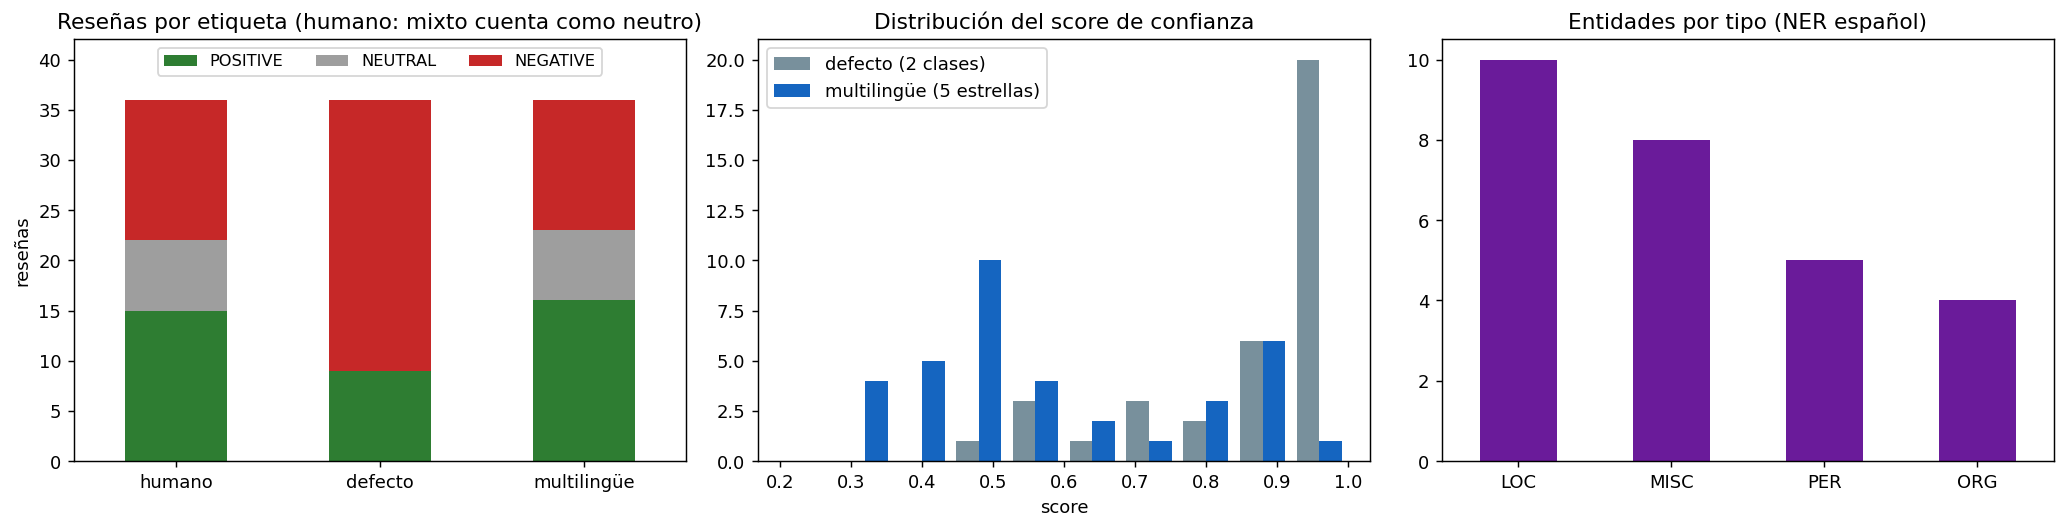
\includegraphics[width=\textwidth]{d_resumen.png}
\end{center}


% ---------------------------------------------------
\section{7. Parte E: análisis de casos difíciles}

Se eligieron \textbf{nueve} reseñas que cubren los tipos de dificultad de la guía: sarcasmo,
negación, opinión mixta, texto muy corto, entidad desconocida, errores ortográficos y score bajo.
Para cada una se registran la predicción, la interpretación humana, si coinciden y la posible causa
del error. \emph{Coinciden} se mide contra el flujo integrado (modelo multilingüe). Si la etiqueta
humana es mixta, cuenta como acierto \texttt{NEUTRAL}; si el modelo o el humano dicen neutro sin
coincidir, se marca como parcial.

\begin{lstlisting}[style=codigo]
import textwrap

CASOS_DIFICILES = {
    # review_id: (tipo de dificultad, interpretación humana, posible causa del error)
    9: ("Sarcasmo",
        "NEGATIVO. Queja por 40 minutos de espera y comida fría; 'genial' e 'inolvidable' son ironía.",
        "Pesan las palabras positivas ('Genial', 'inolvidable') y el modelo no detecta que chocan con "
        "los hechos narrados (40 minutos, llegó fría). Reconocer ironía exige razonamiento pragmático "
        "que un clasificador entrenado con reseñas literales no aprende."),
    # ... 8 casos más con la misma estructura; sus textos completos están
    # en las tablas de abajo y en resultados/e_casos_dificiles.csv
}


def coincidencia(humano, modelo):
    h = MAPA_HUMANO[humano]
    if h == modelo or (h == "MIXED" and modelo == "NEUTRAL"):
        return "Sí"
    if h == "MIXED" or "NEUTRAL" in (h, modelo):
        return "Parcial"
    return "No"


por_id = df.set_index("review_id")
filas = []
for rid, (tipo, humano, causa) in CASOS_DIFICILES.items():
    r = por_id.loc[rid]
    filas.append({
        "review_id": rid,
        "tipo": tipo,
        "text": r["text"],
        "prediccion": f"{r['sentiment']} ({r['sentiment_raw']}, {r['sentiment_score']:.3f})",
        "score_polaridad": r["polarity_score"],
        "prediccion_defecto": f"{r['sentiment_defecto']} ({r['score_defecto']:.3f})",
        "entidades": r["entities"] or "—",
        "interpretacion_humana": humano,
        "coincide": coincidencia(r["etiqueta_humana"], r["sentiment"]),
        "coincide_defecto": coincidencia(r["etiqueta_humana"], r["sentiment_defecto"]),
        "posible_causa": causa,
    })

casos = pd.DataFrame(filas)
casos.to_csv(RESULTADOS / "e_casos_dificiles.csv", index=False)

print("Coincidencia con la interpretación humana")
print("  multilingüe:", casos["coincide"].value_counts().to_dict())
print("  defecto    :", casos["coincide_defecto"].value_counts().to_dict())
casos[["review_id", "tipo", "text", "prediccion", "score_polaridad", "prediccion_defecto", "coincide", "coincide_defecto"]]
\end{lstlisting}

\begin{lstlisting}[style=salida]
Coincidencia con la interpretación humana
  multilingüe: {'No': 5, 'Parcial': 3, 'Sí': 1}
  defecto    : {'No': 7, 'Sí': 1, 'Parcial': 1}
\end{lstlisting}

{\footnotesize\renewcommand{\arraystretch}{1.3}
\begin{longtable}{|>{\raggedright\arraybackslash}p{0.7cm}|>{\raggedright\arraybackslash}p{3.2cm}|>{\raggedright\arraybackslash}p{3.6cm}|>{\raggedright\arraybackslash}p{2.4cm}|>{\raggedright\arraybackslash}p{1.5cm}|>{\raggedright\arraybackslash}p{1.6cm}|}
\hline
\textbf{ID} & \textbf{Tipo} & \textbf{Predicción (multilingüe)} & \textbf{Defecto} & \textbf{Coincide} & \textbf{Coincide def.} \\ \hline
\endfirsthead
\hline
\textbf{ID} & \textbf{Tipo} & \textbf{Predicción (multilingüe)} & \textbf{Defecto} & \textbf{Coincide} & \textbf{Coincide def.} \\ \hline
\endhead
9 & Sarcasmo & POSITIVE (5★, 0.914) & NEGATIVE (0.683) & No & Sí \\ \hline
34 & Sarcasmo con ancla léxica & POSITIVE (5★, 0.945) & POSITIVE (0.553) & No & No \\ \hline
27 & Doble negación & NEGATIVE (2★, 0.559) & NEGATIVE (0.977) & No & No \\ \hline
11 & Negación con sentido positivo (litote) & NEUTRAL (3★, 0.446) & NEGATIVE (0.995) & Parcial & No \\ \hline
23 & Opinión mixta & NEGATIVE (2★, 0.433) & NEGATIVE (0.973) & Parcial & Parcial \\ \hline
13 & Texto muy corto & POSITIVE (5★, 0.324) & POSITIVE (0.985) & No & No \\ \hline
29 & Entidad desconocida + jerga & NEGATIVE (1★, 0.326) & NEGATIVE (0.984) & No & No \\ \hline
16 & Errores ortográficos & POSITIVE (5★, 0.738) & NEGATIVE (0.754) & Sí & No \\ \hline
28 & Negatividad implícita + NER & NEUTRAL (3★, 0.460) & POSITIVE (0.879) & Parcial & No \\ \hline
\end{longtable}}


La celda siguiente del notebook imprime cada caso en detalle. Aquí va en forma de tabla:

\par\noindent\begin{minipage}{\linewidth}\centering\small\renewcommand{\arraystretch}{1.3}
\begin{tabular}{|>{\raggedright\arraybackslash}p{3.1cm}|>{\raggedright\arraybackslash}p{11.9cm}|}
\hline
\multicolumn{2}{|l|}{\textbf{\textcolor{azulUVG}{\#9 · Sarcasmo}}} \\ \hline
\textbf{Reseña} & \emph{Genial, 40 minutos esperando una hamburguesa que llegó fría. Una experiencia inolvidable, de verdad.} \\ \hline
\textbf{Predicción} & POSITIVE (5 estrellas, 0.914); score de polaridad 0.983 \\ \hline
\textbf{Modelo por defecto} & NEGATIVE (0.683) \\ \hline
\textbf{Entidades} & — \\ \hline
\textbf{Interpretación humana} & NEGATIVO. Queja por 40 minutos de espera y comida fría; `genial' e `inolvidable' son ironía. \\ \hline
\textbf{¿Coinciden?} & \textbf{\textcolor{red!70!black}{No}} \\ \hline
\textbf{Posible causa} & Pesan las palabras positivas (`Genial', `inolvidable') y el modelo no detecta que chocan con los hechos narrados (40 minutos, llegó fría). Reconocer ironía exige razonamiento pragmático que un clasificador entrenado con reseñas literales no aprende. \\ \hline
\end{tabular}
\end{minipage}\par\bigskip

\par\noindent\begin{minipage}{\linewidth}\centering\small\renewcommand{\arraystretch}{1.3}
\begin{tabular}{|>{\raggedright\arraybackslash}p{3.1cm}|>{\raggedright\arraybackslash}p{11.9cm}|}
\hline
\multicolumn{2}{|l|}{\textbf{\textcolor{azulUVG}{\#34 · Sarcasmo con ancla léxica}}} \\ \hline
\textbf{Reseña} & \emph{Cinco estrellas... para el aire acondicionado, que es lo único que funcionaba.} \\ \hline
\textbf{Predicción} & POSITIVE (5 estrellas, 0.945); score de polaridad 0.974 \\ \hline
\textbf{Modelo por defecto} & POSITIVE (0.553) \\ \hline
\textbf{Entidades} & — \\ \hline
\textbf{Interpretación humana} & NEGATIVO. Las `cinco estrellas' son para el aire acondicionado, lo único que funcionaba. \\ \hline
\textbf{¿Coinciden?} & \textbf{\textcolor{red!70!black}{No}} \\ \hline
\textbf{Posible causa} & `Cinco estrellas' es casi literalmente la etiqueta `5 stars' con la que se entrenó; en reseñas reales esa frase casi siempre acompaña a una nota de 5. Lo más probable es que el modelo haya aprendido ese atajo y no procese el giro `...para el aire acondicionado'. \\ \hline
\end{tabular}
\end{minipage}\par\bigskip

\par\noindent\begin{minipage}{\linewidth}\centering\small\renewcommand{\arraystretch}{1.3}
\begin{tabular}{|>{\raggedright\arraybackslash}p{3.1cm}|>{\raggedright\arraybackslash}p{11.9cm}|}
\hline
\multicolumn{2}{|l|}{\textbf{\textcolor{azulUVG}{\#27 · Doble negación}}} \\ \hline
\textbf{Reseña} & \emph{No puedo decir que no me haya gustado: el bocadillo de jamón estaba bueno y no tardaron nada.} \\ \hline
\textbf{Predicción} & NEGATIVE (2 estrellas, 0.559); score de polaridad 0.820 \\ \hline
\textbf{Modelo por defecto} & NEGATIVE (0.977) \\ \hline
\textbf{Entidades} & — \\ \hline
\textbf{Interpretación humana} & POSITIVO. `No puedo decir que no me haya gustado' equivale a `me gustó'; `no tardaron nada' es un elogio. \\ \hline
\textbf{¿Coinciden?} & \textbf{\textcolor{red!70!black}{No}} \\ \hline
\textbf{Posible causa} & Tres marcadores negativos (`no', `no', `nada') que el modelo parece sumar como señales negativas en lugar de componerlos: dos negaciones se cancelan y `no tardaron nada' es positivo. \\ \hline
\end{tabular}
\end{minipage}\par\bigskip

\par\noindent\begin{minipage}{\linewidth}\centering\small\renewcommand{\arraystretch}{1.3}
\begin{tabular}{|>{\raggedright\arraybackslash}p{3.1cm}|>{\raggedright\arraybackslash}p{11.9cm}|}
\hline
\multicolumn{2}{|l|}{\textbf{\textcolor{azulUVG}{\#11 · Negación con sentido positivo (litote)}}} \\ \hline
\textbf{Reseña} & \emph{No está nada mal para ser un sitio turístico. Las bravas no tienen nada que envidiar a las de cualquier bar de Les Corts.} \\ \hline
\textbf{Predicción} & NEUTRAL (3 estrellas, 0.446); score de polaridad 0.446 \\ \hline
\textbf{Modelo por defecto} & NEGATIVE (0.995) \\ \hline
\textbf{Entidades} & LOC:Les Corts (1.00) \\ \hline
\textbf{Interpretación humana} & POSITIVO. `No está nada mal' y `no tienen nada que envidiar' son elogios. \\ \hline
\textbf{¿Coinciden?} & \textbf{\textcolor{orange!80!black}{Parcial}} \\ \hline
\textbf{Posible causa} & Acumula `no', `nada', `mal' y `envidiar'. El modelo duda (3 estrellas) y no llega a invertir la polaridad: sumando 4 y 5 estrellas la probabilidad positiva es 0.48, apenas por encima del 0.45 neutro. \\ \hline
\end{tabular}
\end{minipage}\par\bigskip

\par\noindent\begin{minipage}{\linewidth}\centering\small\renewcommand{\arraystretch}{1.3}
\begin{tabular}{|>{\raggedright\arraybackslash}p{3.1cm}|>{\raggedright\arraybackslash}p{11.9cm}|}
\hline
\multicolumn{2}{|l|}{\textbf{\textcolor{azulUVG}{\#23 · Opinión mixta}}} \\ \hline
\textbf{Reseña} & \emph{Los camareros son un amor, pero la cocina es un desastre: el pollo seco y las patatas congeladas.} \\ \hline
\textbf{Predicción} & NEGATIVE (2 estrellas, 0.433); score de polaridad 0.653 \\ \hline
\textbf{Modelo por defecto} & NEGATIVE (0.973) \\ \hline
\textbf{Entidades} & — \\ \hline
\textbf{Interpretación humana} & MIXTO. Servicio excelente (`un amor') y cocina muy mala (`un desastre'). \\ \hline
\textbf{¿Coinciden?} & \textbf{\textcolor{orange!80!black}{Parcial}} \\ \hline
\textbf{Posible causa} & Una sola etiqueta no puede expresar dos aspectos opuestos. El modelo pesa más la cláusula que sigue al `pero' y da 2 estrellas; el score bajo refleja la mezcla. Haría falta análisis de sentimiento por aspectos (servicio / comida / precio; Pontiki et al., 2014). \\ \hline
\end{tabular}
\end{minipage}\par\bigskip

\par\noindent\begin{minipage}{\linewidth}\centering\small\renewcommand{\arraystretch}{1.3}
\begin{tabular}{|>{\raggedright\arraybackslash}p{3.1cm}|>{\raggedright\arraybackslash}p{11.9cm}|}
\hline
\multicolumn{2}{|l|}{\textbf{\textcolor{azulUVG}{\#13 · Texto muy corto}}} \\ \hline
\textbf{Reseña} & \emph{Carísimo.} \\ \hline
\textbf{Predicción} & POSITIVE (5 estrellas, 0.324); score de polaridad 0.544 \\ \hline
\textbf{Modelo por defecto} & POSITIVE (0.985) \\ \hline
\textbf{Entidades} & — \\ \hline
\textbf{Interpretación humana} & NEGATIVO. Una sola palabra que critica el precio. \\ \hline
\textbf{¿Coinciden?} & \textbf{\textcolor{red!70!black}{No}} \\ \hline
\textbf{Posible causa} & Sin contexto, y con un vocabulario multilingüe que trocea la palabra en `car' + `\#\#isi' + `\#\#mo', el modelo no tiene señal. Su score es de los más bajos del lote: avisa que no sabe. El modelo por defecto, en cambio, se equivoca con 0.985. \\ \hline
\end{tabular}
\end{minipage}\par\bigskip

\par\noindent\begin{minipage}{\linewidth}\centering\small\renewcommand{\arraystretch}{1.3}
\begin{tabular}{|>{\raggedright\arraybackslash}p{3.1cm}|>{\raggedright\arraybackslash}p{11.9cm}|}
\hline
\multicolumn{2}{|l|}{\textbf{\textcolor{azulUVG}{\#29 · Entidad desconocida + jerga}}} \\ \hline
\textbf{Reseña} & \emph{La Blaugrana Burger con salsa Culé está brutal, pídanla sin dudar.} \\ \hline
\textbf{Predicción} & NEGATIVE (1 estrella, 0.326); score de polaridad 0.577 \\ \hline
\textbf{Modelo por defecto} & NEGATIVE (0.984) \\ \hline
\textbf{Entidades} & MISC:Blaugrana Burger (1.00); MISC:Culé (1.00) \\ \hline
\textbf{Interpretación humana} & POSITIVO. En España `brutal' significa `buenísimo'; `Blaugrana Burger' y `salsa Culé' son productos. \\ \hline
\textbf{¿Coinciden?} & \textbf{\textcolor{red!70!black}{No}} \\ \hline
\textbf{Posible causa} & El sentido normativo de `brutal' (cruel, violento), que coincide con el inglés, es negativo y probablemente es el que dominó en el entrenamiento. Los nombres inventados no aportan señal. En NER, con `simple' `Culé' salía partido en `Cul' + `é'; con `first' ambos productos quedan como MISC. \\ \hline
\end{tabular}
\end{minipage}\par\bigskip

\par\noindent\begin{minipage}{\linewidth}\centering\small\renewcommand{\arraystretch}{1.3}
\begin{tabular}{|>{\raggedright\arraybackslash}p{3.1cm}|>{\raggedright\arraybackslash}p{11.9cm}|}
\hline
\multicolumn{2}{|l|}{\textbf{\textcolor{azulUVG}{\#16 · Errores ortográficos}}} \\ \hline
\textbf{Reseña} & \emph{q buen sitio!! los nachos buenisimos y el camarero super atento, bolveremos seguro} \\ \hline
\textbf{Predicción} & POSITIVE (5 estrellas, 0.738); score de polaridad 0.966 \\ \hline
\textbf{Modelo por defecto} & NEGATIVE (0.754) \\ \hline
\textbf{Entidades} & — \\ \hline
\textbf{Interpretación humana} & POSITIVO. Elogio claro pese a `q', `buenisimos' y `bolveremos'. \\ \hline
\textbf{¿Coinciden?} & \textbf{\textcolor{verde}{Sí}} \\ \hline
\textbf{Posible causa} & Coincide. Las faltas no borran las señales fuertes (`buen sitio', `super atento', `!!') y el modelo es uncased y quita acentos, así que `buenisimos' y `buenísimos' se tokenizan igual. El modelo por defecto falla porque no conoce el español. \\ \hline
\end{tabular}
\end{minipage}\par\bigskip

\par\noindent\begin{minipage}{\linewidth}\centering\small\renewcommand{\arraystretch}{1.3}
\begin{tabular}{|>{\raggedright\arraybackslash}p{3.1cm}|>{\raggedright\arraybackslash}p{11.9cm}|}
\hline
\multicolumn{2}{|l|}{\textbf{\textcolor{azulUVG}{\#28 · Negatividad implícita + NER}}} \\ \hline
\textbf{Reseña} & \emph{Esperaba algo digno del Museu del Barça y me encontré un bar de aeropuerto con precios de Plaça de Catalunya.} \\ \hline
\textbf{Predicción} & NEUTRAL (3 estrellas, 0.460); score de polaridad 0.460 \\ \hline
\textbf{Modelo por defecto} & POSITIVE (0.879) \\ \hline
\textbf{Entidades} & MISC:Museu del Barça (0.69); LOC:Catalunya (0.97) \\ \hline
\textbf{Interpretación humana} & NEGATIVO. Compara el local con un bar de aeropuerto con precios de zona turística. \\ \hline
\textbf{¿Coinciden?} & \textbf{\textcolor{orange!80!black}{Parcial}} \\ \hline
\textbf{Posible causa} & No hay palabras negativas: la crítica está en la comparación, y entenderla requiere saber que un `bar de aeropuerto' es caro y mediocre. El modelo queda en 3 estrellas. En NER, `Plaça de Catalunya' se reduce a `Catalunya' y con `simple' `Museu' salía partido en `Muse' + `u'. \\ \hline
\end{tabular}
\end{minipage}\par\bigskip

\subsection{Patrones que dejan los casos difíciles}

\begin{enumerate}[leftmargin=1.4em]
\item
  \textbf{El score no protege contra el sarcasmo.} Las dos predicciones con mayor score de todo el
  lote (\#34 con 0.945 y \#9 con 0.914) son sarcasmos clasificados como 5 estrellas. El modelo está
  más seguro justo cuando más se equivoca.
\item
  \textbf{La negación se lee como vocabulario, no como operador.} ``No está nada mal'' (\#11) y
  ``no puedo decir que no me haya gustado'' (\#27) contienen varias palabras negativas y el modelo las
  acumula en vez de invertir su efecto. El modelo por defecto falla las dos con scores de 0.99 y 0.98.
\item
  \textbf{Cuando falta señal, el modelo sí lo avisa.} En el texto de una palabra (\#13), en la reseña
  informativa (\#17) y en la crítica implícita (\#28) el score cae por debajo de 0.5. En esos casos el
  score funciona como alarma útil.
\item
  \textbf{Robusto a faltas, frágil ante la jerga.} Las reseñas con errores ortográficos (\#15 y \#16) se
  clasifican bien, pero una sola palabra de uso regional (``brutal'', \#29) invierte la predicción.
\item
  \textbf{En NER hay dos tipos de error.} Los de \emph{agregación} (entidades partidas en subpalabras)
  desaparecen con \texttt{first}. Los de \emph{etiquetado} se quedan: una persona pública marcada como \texttt{MISC},
  una entidad truncada y un falso positivo por mayúscula inicial.
\end{enumerate}


% ---------------------------------------------------
\section{8. Preguntas de reflexión}

\subsection{1. ¿El modelo parece apropiado para reseñas en español?}

\textbf{El modelo por defecto, no.} \texttt{distilbert-base-uncased-finetuned-sst-2-english} se entrenó con
reseñas de cine en inglés. Sobre las 36 reseñas predijo \texttt{NEGATIVE} en 27, acertó el \textbf{55 \%} de
las polares (apenas mejor que una moneda) y solo reconoció \textbf{1 de cada 3} positivas (recall 0.33).
Sus predicciones positivas más seguras son justo las dos reseñas con palabras en inglés (``Top!!'' y
``Amazing\ldots{} very friendly'', ambas con 0.9998).
Lo más problemático es que falla con seguridad: su score promedio es 0.87.

\textbf{El modelo multilingüe es aceptable como primer filtro, pero no es ideal.}
\texttt{nlptown/bert-base-multilingual-uncased-sentiment} sí vio reseñas en español y llega al \textbf{72 \%} de
acierto, con F1 de 0.80 en positivas y 0.72 en negativas. Aun así se entrenó con reseñas de
\emph{producto}, no de restaurantes, y no conoce la jerga de España. El siguiente paso sería un modelo
nativo en español (en una prueba exploratoria con seis frases,
\texttt{pysentimiento/robertuito-sentiment-analysis} (Pérez et al., 2021) resolvió mejor ``no está mal'' pero también cayó en
el sarcasmo) o, mejor, afinar con unos cientos de reseñas de restaurantes etiquetadas.

\subsection{2. ¿Qué errores de sentimiento encontraste?}

\begin{itemize}[leftmargin=1.2em]
\item
  \textbf{Sarcasmo} clasificado como positivo y con el score más alto del lote (\#9, \#34).
\item
  \textbf{Negación compuesta:} litote (\#11 → 3 ★) y doble negación (\#27 → 2 ★).
\item
  \textbf{Jerga regional:} ``está brutal'' leído como negativo (\#29 → 1 ★).
\item
  \textbf{Texto muy corto:} ``Carísimo.'' → 5 ★ (\#13), aunque con score bajo.
\item
  \textbf{Reseña informativa} sin opinión (\#17) → 5 ★. El modelo no tiene clase ``sin opinión'': todas las
  reseñas con las que se entrenó valoran algo.
\item
  \textbf{Crítica implícita} por comparación (\#28 → 3 ★).
\item
  \textbf{Mixtas:} tres de cinco caen en 3 ★ y dos en 2 ★. Es razonable, pero pierde el aspecto positivo.
\item
  \textbf{Sesgo del modelo por defecto:} casi todo lo que no entiende lo manda a \texttt{NEGATIVE}, y así acierta
  negativas ``por accidente''.
\end{itemize}

\subsection{3. ¿Qué problemas observaste en NER?}

\begin{itemize}[leftmargin=1.2em]
\item
  \textbf{Fragmentación en subpalabras} con \texttt{aggregation\_strategy="simple"}: 8 fragmentos de 32 entidades
  en el modelo en español (\texttt{Nu}+\texttt{ria}, \texttt{Spo}+\texttt{tify\ Camp\ Nou}) y 22 de 46 en el modelo por defecto.
  Con \texttt{first} bajan a 0.
\item
  \textbf{Falsos positivos del modelo en inglés} sobre palabras en mayúscula o trozos de palabras:
  \texttt{del} → LOC, \texttt{ca} → PER, \texttt{Me} (de ``Meh.'') → PER, \texttt{Carís} → ORG, y \texttt{mb}/\texttt{ues} → MISC dentro de
  ``hamburguesa(s)'' (posiblemente por su parecido con \emph{Hamburg}).
\item
  \textbf{Tipo equivocado:} \texttt{Lamine\ Yamal} sale como \texttt{MISC} y no como \texttt{PER}.
\item
  \textbf{Entidades truncadas:} \texttt{Plaça\ de\ Catalunya} → \texttt{Catalunya}; de ``los hermanos Iglesias'' solo queda
  \texttt{Iglesias}, que además es un sustantivo común.
\item
  \textbf{Mayúscula = entidad:} \texttt{Ambiente\ único} se marca \texttt{MISC} solo por empezar oración.
\item
  \textbf{Categorías que no encajan en el dominio:} CoNLL-2002 son noticias. No existe una clase para
  platos o productos (\texttt{Blaugrana\ Burger} cae en \texttt{MISC}), y \texttt{Spotify\ Camp\ Nou} es a la vez estadio
  (LOC) y marca patrocinada (ORG), así que el modelo lo manda a \texttt{MISC}.
\item
  \textbf{Lo que funcionó:} los cuatro nombres ficticios de personas (Nuria, Santiago, Mateo, Sergi) y las
  organizaciones y países se detectaron, todos con score superior a 0.9.
\end{itemize}

\subsection{4. ¿Cómo influye el score en tu confianza?}

El score es la probabilidad softmax de la clase ganadora, \textbf{no la probabilidad de acertar}.

\begin{itemize}[leftmargin=1.2em]
\item
  En el modelo por defecto, de las 23 predicciones polares con score \textgreater{} 0.8 solo acertó el \textbf{61 \%}.
\item
  En el multilingüe, el rango de score \textgreater{} 0.8 acierta menos (75 \%) que el de 0.5--0.8 (89 \%), porque
  ahí están los dos sarcasmos.
\item
  Con cinco clases el score de la estrella ganadora \textbf{subestima} la confianza: \#24 es claramente
  positiva, acierta y tiene 0.30, porque el resto de la probabilidad se fue a 4 estrellas. Sumando la
  polaridad sube a 0.55. Ese \texttt{score\_polaridad} se comporta mejor: 82 \% de acierto por encima de 0.8
  y 0 \% por debajo de 0.5 (aunque ese rango solo tiene 3 reseñas).
\end{itemize}

Conclusión: \textbf{un score bajo es una buena alarma} para mandar la reseña a revisión humana, pero \textbf{un
score alto no es garantía}. Además no es comparable entre modelos con distinto número de clases, y
saber si está calibrado exige datos etiquetados.

\subsection{5. ¿Qué datos etiquetarías manualmente para calcular precision, recall y F1?}

\textbf{Sentimiento}

\begin{itemize}[leftmargin=1.2em]
\item
  Una muestra \textbf{estratificada} de reseñas reales: todas las estrellas, idiomas y longitudes, y
  sobremuestreo de los casos difíciles (sarcasmo, negación, mixtas), porque son raros pero caros.
\item
  Al menos 200--300 reseñas, para tener unas 30 por clase aun con la distribución real, que es muy
  polarizada (176 / 33 / 34 / 44 / 137).
\item
  Etiquetas \texttt{POSITIVO} / \texttt{NEGATIVO} / \texttt{NEUTRO} / \texttt{MIXTO} y marcas de fenómeno, asignadas por \textbf{dos
  anotadores} con una guía escrita, midiendo su acuerdo (kappa de Cohen, 1960). Las estrellas del usuario
  sirven como señal débil, pero no reemplazan la etiqueta: la nota y el texto no siempre coinciden.
\item
  Reportar \textbf{F1 macro}, porque las clases están desbalanceadas.
\end{itemize}

En este laboratorio ya se hizo una versión mínima: la columna \texttt{etiqueta\_humana} permitió calcular
las métricas de la Parte D.4.

\textbf{NER}

\begin{itemize}[leftmargin=1.2em]
\item
  Spans exactos con su tipo, siguiendo una guía que decida de antemano los casos ambiguos: estadio =
  LOC, Barça Cafe = ORG, platos = una clase \texttt{PRODUCTO} nueva y figuras públicas = PER.
\item
  Evaluación \textbf{a nivel de entidad} (coincidencia exacta de span y tipo, como \texttt{seqeval}; Nakayama, 2018), y aparte
  las coincidencias parciales para cuantificar las truncaciones (\texttt{Catalunya} vs.~\texttt{Plaça\ de\ Catalunya}).
\end{itemize}

\subsection{6. ¿Usarías estas predicciones para tomar decisiones automáticas importantes? ¿Por qué?}

\textbf{No.}

\begin{itemize}[leftmargin=1.2em]
\item
  El 72 \% de acierto sale de 29 reseñas: la muestra es pequeña y el margen de error, amplio.
\item
  Los errores \textbf{no son aleatorios}: se concentran en sarcasmo y negación, que abundan justo en las
  reseñas enojadas, las que más importan.
\item
  Los errores más graves llegan con score alto, así que un umbral de confianza no los filtra.
\item
  El NER extrae nombres de empleados (``el encargado Sergi''). Tomar decisiones sobre personas a
  partir de eso tiene implicaciones laborales y de privacidad.
\end{itemize}

Sí lo usaría como \textbf{apoyo}, con una persona en el circuito:

\begin{itemize}[leftmargin=1.2em]
\item
  \textbf{Tendencias agregadas}, por ejemplo el porcentaje de reseñas negativas por mes o por tema. Ahí
  los errores individuales se compensan y basta con una auditoría humana periódica.
\item
  \textbf{Triaje:} mandar a revisión humana primero lo \texttt{NEGATIVE} o con score de polaridad bajo.
\end{itemize}

No lo usaría para responder públicamente de forma automática, borrar reseñas, fijar precios ni
evaluar o sancionar a un empleado mencionado.


% ---------------------------------------------------
\section{Conclusiones}

\begin{enumerate}[leftmargin=1.4em]
\item \textbf{El modelo por defecto no es una opción para español.} La llamada literal de la guía
elige un modelo de reseñas de cine en inglés. Acierta el 55\,\% de las reseñas polares, marca como
negativas 27 de 36 y lo hace con un score promedio de 0.87. Hay que elegir el modelo explícitamente.

\item \textbf{Un modelo multilingüe entrenado con reseñas mejora mucho, pero falla donde más
importa.} Llega al 72\,\% de acierto, con F1 de 0.80 y 0.72, y sus errores no son aleatorios: se
concentran en sarcasmo, negación compuesta y jerga, que abundan en las reseñas enojadas.

\item \textbf{El score sirve como alarma, no como garantía.} Un score bajo sí señala dudas (tres de
las cinco reseñas menos seguras son errores). Pero las dos predicciones más seguras del lote son
sarcasmos mal clasificados. Con cinco clases conviene sumar la probabilidad por polaridad antes de
interpretarlo.

\item \textbf{En NER, la configuración pesa tanto como el modelo.} Cambiar la estrategia de
agregación de \texttt{simple} a \texttt{first} eliminó los ocho fragmentos de subpalabras sin
tocar el modelo. Los errores que quedan (tipo equivocado, entidades truncadas,
falsos positivos por mayúscula) sí requieren datos del dominio para corregirse.
\end{enumerate}

% ---------------------------------------------------
\section{Referencias}

\begin{referencias}

\item Cañete, J., Chaperon, G., Fuentes, R., Ho, J.-H., Kang, H., \& Pérez, J. (2020).
\emph{Spanish pre-trained BERT model and evaluation data}. PML4DC Workshop at ICLR 2020.
\url{https://github.com/dccuchile/beto}

\item Cohen, J. (1960). A coefficient of agreement for nominal scales. \emph{Educational and
Psychological Measurement, 20}(1), 37--46. \url{https://doi.org/10.1177/001316446002000104}

\item Devlin, J., Chang, M.-W., Lee, K., \& Toutanova, K. (2019). BERT: Pre-training of deep
bidirectional transformers for language understanding. En \emph{Proceedings of NAACL-HLT 2019}
(pp. 4171--4186). Association for Computational Linguistics.
\url{https://doi.org/10.18653/v1/N19-1423}

\item FC Barcelona. (2021). \emph{Barça Cafe, the new emblematic restaurant at Camp Nou}.
\url{https://www.fcbarcelona.com/en/news/2139272/barca-cafe-the-new-emblematic-restaurant-at-camp-nou}

\item Google. (s.f.). \emph{Barça Cafe} [Ficha y opiniones en Google Maps]. Recuperado el 14 de
septiembre de 2026 de \url{https://www.google.com/maps/search/Barca+Cafe+Barcelona}

\item Guo, C., Pleiss, G., Sun, Y., \& Weinberger, K. Q. (2017). On calibration of modern neural
networks. En \emph{Proceedings of the 34th International Conference on Machine Learning}
(pp. 1321--1330). PMLR.

\item Hugging Face. (s.f.). \emph{Pipelines: TokenClassificationPipeline}. Transformers
Documentation. \url{https://huggingface.co/docs/transformers/main_classes/pipelines}

\item Nakayama, H. (2018). \emph{seqeval: A Python framework for sequence labeling evaluation}
[Software]. \url{https://github.com/chakki-works/seqeval}

\item NLP Town. (s.f.). \emph{bert-base-multilingual-uncased-sentiment} [Modelo]. Hugging Face.
\url{https://huggingface.co/nlptown/bert-base-multilingual-uncased-sentiment}

\item Pérez, J. M., Rajngewerc, M., Giudici, J. C., Furman, D. A., Luque, F., Alonso Alemany, L.,
\& Martínez, M. V. (2021). \emph{pysentimiento: A Python toolkit for opinion mining and social NLP
tasks}. arXiv. \url{https://arxiv.org/abs/2106.09462}

\item Pontiki, M., Galanis, D., Pavlopoulos, J., Papageorgiou, H., Androutsopoulos, I., \&
Manandhar, S. (2014). SemEval-2014 Task 4: Aspect based sentiment analysis. En \emph{Proceedings
of the 8th International Workshop on Semantic Evaluation} (pp. 27--35). Association for
Computational Linguistics. \url{https://doi.org/10.3115/v1/S14-2004}

\item Romero, M. (s.f.). \emph{bert-spanish-cased-finetuned-ner} [Modelo]. Hugging Face.
\url{https://huggingface.co/mrm8488/bert-spanish-cased-finetuned-ner}

\item Sanh, V., Debut, L., Chaumond, J., \& Wolf, T. (2019). \emph{DistilBERT, a distilled version
of BERT: Smaller, faster, cheaper and lighter}. arXiv. \url{https://arxiv.org/abs/1910.01108}

\item Socher, R., Perelygin, A., Wu, J., Chuang, J., Manning, C. D., Ng, A., \& Potts, C. (2013).
Recursive deep models for semantic compositionality over a sentiment treebank. En
\emph{Proceedings of the 2013 Conference on Empirical Methods in Natural Language Processing}
(pp. 1631--1642). Association for Computational Linguistics.

\item Tjong Kim Sang, E. F. (2002). Introduction to the CoNLL-2002 shared task:
Language-independent named entity recognition. En \emph{Proceedings of CoNLL-2002}.
\url{https://aclanthology.org/W02-2024/}

\item Tjong Kim Sang, E. F., \& De Meulder, F. (2003). Introduction to the CoNLL-2003 shared task:
Language-independent named entity recognition. En \emph{Proceedings of CoNLL-2003} (pp. 142--147).
\url{https://aclanthology.org/W03-0419/}

\item Wolf, T., Debut, L., Sanh, V., Chaumond, J., Delangue, C., Moi, A., Cistac, P., Rault, T.,
Louf, R., Funtowicz, M., Davison, J., Shleifer, S., von Platen, P., Ma, C., Jernite, Y., Plu, J.,
Xu, C., Le Scao, T., Gugger, S., \ldots{} Rush, A. (2020). Transformers: State-of-the-art natural
language processing. En \emph{Proceedings of the 2020 Conference on Empirical Methods in Natural
Language Processing: System Demonstrations} (pp. 38--45). Association for Computational
Linguistics. \url{https://doi.org/10.18653/v1/2020.emnlp-demos.6}

\end{referencias}

\end{document}
